
% \documentclass[nobib,a4,twosided,justified,symmetric]{tufte-book}
\documentclass[nobib,a4,twosided,justified]{tufte-book}
\usepackage[english,brazilian]{babel}
\usepackage[utf8]{inputenc}
\usepackage[T1]{fontenc}
\usepackage{csquotes}
\usepackage{cabin}
\usepackage{tgpagella}
\usepackage{hyphenat}
\usepackage[citetracker=constrict,style=authoryear,autocite=footnote]{biblatex}
% \usepackage[backend=bibtex,autocite=footnote,style=alphabetic]{biblatex}
\addbibresource{./document.bib}
\usepackage{lipsum}
\usepackage{booktabs}
\usepackage{graphicx}
\usepackage[fleqn,tbtags]{amsmath}
\usepackage{mathtools}
\usepackage{amsfonts}
\usepackage{eucal}
\usepackage{mathrsfs}
\usepackage{epigraph}
\usepackage{etoolbox}
\usepackage[amsmath,thmmarks]{ntheorem}
\setkeys{Gin}{width=\linewidth,totalheight=\textheight,keepaspectratio}
\graphicspath{{./graphics/}}
\usepackage{makeidx}
\makeindex
% \usepackage[nodisplayskipstretch]{setspace}
% \setstretch{1.5}

\usepackage{style}  % my macros and other tunes
% \allowdisplaybreaks[1]
% \setlength{\belowdisplayskip}{0pt} \setlength{\belowdisplayshortskip}{0pt}
% \setlength{\abovedisplayskip}{0pt} \setlength{\abovedisplayshortskip}{0pt}
%% \makeatletter

%% \let\orig@maketag@@@\maketag@@@
%% \renewcommand{\eqref}[1]{\textup{\let\maketag@@@\orig@maketag@@@\tagform@{\ref{#1}}}}

%% \def\maketag@@@#1{\hbox{\rlap{\kern\marginparsep\m@th\normalfont#1}\kern1sp}}
%% \makeatother


\newcommand{\blankpage}{\newpage\hbox{}\thispagestyle{empty}\newpage}

\hypersetup{colorlinks}  % hyperlinks coloridos

%%% Metadata {{}
\title{%
    Quebra de Simetria Espontânea,
     \\Limites Cognitivos e
     \\Complexidade de Sociedades
}
\author{Felippe Alves Pereira}
\publisher{Instituto de Física - Universidade de São Paulo}
%%%

%%% Document
\begin{document}

%%% front matter
\frontmatter

%\chapter*{Dedicatória}
%\chapter*{Declaração}

\blankpage

\cleardoublepage%
{%
\begin{fullwidth}%

\centering{
    \fontsize{18}{28}\selectfont\par\noindent{Universidade de São Paulo\\Instituto de Física}%
    \vspace{1.25in}%


    \fontsize{24}{30}\selectfont\par\noindent{Quebra de Simetria Espontânea,\\Limites Cognitivos e\\Complexidade de Sociedades\\}%
    \vspace{2cm}%
    % \LARGE\par\noindent\edition%
    % \vfill%
    \fontsize{20}{30}\selectfont\par\noindent{Felippe Alves Pereira\\}%
    }
    \vspace{2cm}
    \flushright{
    {\fontsize{14}{20}\selectfont\par\noindent{Orientador: Prof.Dr. Nestor Caticha\\}}
        \vspace{1cm}
        Dissertação de Mestrado apresentada\\ao Instituto de Física para a obtenção\\do título de Mestre em Ciências
    }
    \vspace{1cm}
    \flushleft{
        Banca Examinadora:

        Prof.Dr.\\
        Prof.Dr.\\
        Prof.Dr.\\
    }
    \vfill
    \centering{São Paulo - 2015}

    \end{fullwidth}%
}
    \thispagestyle{empty}%
    \clearpage%

%\maketitle
% \newpage

\chapter*{Agradecimentos}

Agradeço a meus pais e ao meu irmão pelo apoio dado e confiança em mim depositada.
Agradeço ao Nestor Caticha pela orientação e pelo entusiasmo.
Agradeço à Milena pela preocupação, paciência e pelos ouvidos.
\blankpage

\chapter*{Resumo}

Neste trabalho elaboramos um modelo para a formação de estruturas sociais através das características cognitivas das pessoas e do modo como interagem umas com as outras.
Com base em estudos nos campos da neurociência e da psicologia social, além do uso das técnicas de mecânica estatística e da teoria de aprendizado de máquina, fomos capazes de estabelecer um modelo de agentes que trocam opiniões, aprendem e escolhem seus parceiros com base nas informações que obtêm.

A dinâmica das relações sociais introduzida aqui é capaz de produzir complexidade na estrutura das relações sociais e na distribuição de opiniões de forma correlacionada.
Essa dinâmica nos dá um parâmetro que mede o nível de organização social e nos permite interpretar o fenômeno de formação de comunidades como uma estrutura que requer uma \emph{"massa crítica"} para se estabelecer.

Com base nesses resultados, propusemos um modelo capaz de reproduzir parte do comportamento observado no plenário brasileiro ao londo do anos em relação a votações de projetos de lei sob diferentes mandatos presidenciais.

\chapter*{Abstract}

In this work we establish a model for social structure formation based on cognitive characteristics of human beings and how they interact with each other.
From neuroscience and social psychology studies, and also relying on technique from statistical mechanics and machine leaning theory, we were able to establish a model of agents who exchange opinions, learn together and choose their partnerships using the information they gather.

The social relationship dynamics here introduced is capable of generating complexity on the social structure level and a on opinion distribution in a correlated way.
This dynamics gives a parameter representing the degree to which society is organized and allow us to see the phenomena of community formation as a structure requiring a \emph{"critical mass"} to fixate.

These results guided us in proposing a model able to replicate a portion of the behavior observed at the Brazilian plenary through year of voting law projects under different president mandates.

\tableofcontents
% \listoffigures
% \listoftables
%%%

%%% main matter
\mainmatter
% ideia
% cap 1 : apresentação dos modelos, interpretação de beta
% cap 2 : dinâmica de reputação
% cap 3 : campo médio e a desconfiança
% cap 4 : jogos de partidos
% ESSA ESTRUTURA NÃO É MANDATÓRIA, SÓ UMA GUIA!
% OS NOMES DOS CAPÍTULOS NÃO SERÃO ESTES, NECESSÁRIAMENTE.

%% Capítulo 1

%%% Capítulo 1 - Introdução

\chapter{Um Panorama do Estudo\\de Fenômenos Sociais}
\label{ch:C1}
\chapquote{
... I can see no other escape from this dilemma (lest our true aim be  lost for ever) than that some of us should venture to embark on a synthesis  of facts and theories, albeit with second-hand and incomplete knowledge of some of them, and at the risk of making fool of ourselves.
So much for my apology.
}{Erwin Schrödinger, \emph{What is Life?} (1944)}

Os conceitos de fenômeno social e de natureza humana se entrelaçam.
A complexidade e diversidade observadas na sociedade despertam o interesse de cientistas em diferentes campos, dedicados a questionar e entender os mecanismos que as produzem.
É possível, por exemplo, que um sociólogo se interesse em entender como diferentes grupos lidam com resolução de conflitos, enquanto um psicólogo esteja preocupado com a abordagem de cada indivíduo envolvido numa situação de conflito, um neurocientista queira analisar a ativação cerebral em cada abordagem descrita pelo psicólogo, um estatístico queira entender as correlações entre estrutura social e comportamento, e a um físico talvez caiba tentar entender a dinâmica que rege esse tipo de fenômeno.

Uma característica, talvez a mais interessante, de sistemas sociais é a exibição simultânea de estruturas organizadas e ricas em diversidade.
Embora as pessoas tendam a reproduzir o comportamento de seus pares, ainda observamos diversidade cultural, formação de estados e dialetos num mesmo idioma por exemplo.
O estudo dessa característica das sociedades humanas tem sido abordada por diferentes estratégias na pesquisa contemporânea.

Nesse contexto, o psicólogo social \emph{J. Haidt} e seus colegas na formulação da \emph{Teoria dos Fundamentos Morais} \footcite{Haidt2007,Graham2011} estabeleceram as bases para relacionar a resposta neural de indivíduos em questões de conflito moral com a participação deste na manutenção da sociedade.
Através de resultados sobre o aprendizado de comportamento moral, da intuitividade dos julgamentos e do mapeamento da moral, a Teoria dos Fundamentos Morais, propõe que o domínio da moralidade humana não é composto apenas por questões relacionadas ao modo como dois indivíduos devam se tratar, mas também por características que dizem respeito ao papel do indivíduo no grupo.
Além disso, a diversidade encontrada no conceito de moral através das culturas pode ser explicada tomando a moral como um conjunto de mecanismos, biológicos ou culturais, que regulam o egoísmo e tornam a vida social possível.
Essa linha de pensamento contribui para a compreensão da complexidade social na escala das interações humanas e será um ponto de partida útil na elaboração dos modelos estudados neste trabalho.

Numa perspectiva mais coletivista, \emph{R. Axelrod} \footcite{Axelrod1997} propôs um modelo qualitativo para a diversidade cultural em termos de agentes interagentes, no qual ele foi capaz de mostrar a possibilidade da coexistência de diferentes culturas numa dada região como uma consequência da homofilia local.
Nesse modelo, a capacidade de interagir com maior probabilidade com agentes mais parecidos é capaz de produzir fronteiras separando regiões de agentes que são compatíveis e incompatíveis.
Esse resultado é interessante por si, mas o modelo deixa aberto generalizações em diversos sentidos como a topologia do grafo onde os agentes interagem e o efeito das particularidades no mecanismo de aprendizado.

O uso de modelos de agentes em grafos tem sido amplamente empregado no estudo de sistemas sociais.
O presente trabalho se insere numa série de outros no esforço de entender melhor o papel das características humanas na constituição das estruturas sociais.
Integram essa série, modelos relacionando o aprendizado moral com as estruturas cognitivas da interação de indivíduos \footcite{Caticha2011,Vicente2014,Cesar2014} e modelos de surgimento de autoridade e desenvolvimento econômico \footcite{Papa2014,Calsaverini2013}.

O ponto em comum nesses trabalhos recentes são algumas bases empíricas que proporcionam a abordagem de comportamentos sociais como consequência das capacidade humana de aprendizado, das respostas neurológicas a dilemas morais e conflitos sociais ou nas escolhas de estratégias, das estruturas de informação provenientes das interações sociais e de uma compreensão um pouco mais ampla dos processos de aprendizado.

A exploração dos fenômenos sociais como consequência das características psico ou neurológicas dos indivíduos distingue esses recentes esforços das linhas mais \emph{`cinemáticas`} de estudo \footcite{Castellano2009}.
Em outras palavras, além da descrição de como um certo fenômeno ocorre são interessantes também as causas desse fenômeno.
Seguiremos, então, com uma breve apresentação das motivações empíricas sobre o comportamento humano e sua possível influência nas construções sociais.

\section{Aprendizado por Reforço}

Uma das características, não exclusivamente, humanas é sua capacidade de aprender através do sucesso ou do fracasso.
Somos capazes de aprender comportamento, criar abstrações e fazer previsões com base em experiência prévia em diversas circunstâncias.
Embora essa afirmação não seja chocante em si, talvez surpreenda o fato de que estamos aprendendo como funcionam nossos mecanismos de aprendizado, a nível neurológico, psicológico e social.

Um desses mecanismos é o de aprendizado por reforço, ou em outras palavras a habilidade de aprender com erros e acertos.
Para isso é necessário que tenhamos aparatos neurais para planejar uma ação, prever o resultado e detectar erros na previsão para poder ajustar uma próxima ação.

Estudos realizados por \parencite{Holroyd2002a} mostram como o mecanismo de as regiões do Córtex Cingulado Anterior \footnote{tradução livre de \emph{Anterior Cingulate Cortex}(ACC)} em conjunto com os sistemas dopaminérgicos do mesencéfalo funcionam como um mecanismo de detecção de erros e recompensas durante o aprendizado de uma tarefa.
Esse mecanismo é estudado através da análise de eletroencefalograma, mais especificamente na ocorrência de Negatividade Relacionada ao Erro \footnote{tradução livre de \emph{Error-Related Negativity} (ERN)}.
A existência de tal mecanismo de aprendizado por reforço é uma das bases que fundamenta o uso da teoria de aprendizado de máquina para modelar o comportamento social.

A tarefa de detectar conflitos exercida pelo córtex cingulado anterior está diretamente relacionada à sensação de dor física.
Em paralelo à capacidade de aprendizado, os estudos de \parencite{Somerville2006,Eisenberger2003} apontam um aumento na atividade do córtex cingulado anterior quando um indivíduo vivencia exclusão social ou é avaliado negativamente por outras pessoas.
O fato da região do cérebro responsável pela dor física também ser ativada durante a experiência de conflitos sociais sugere que há um custo, talvez análogo à dor física, a ser pago ao se envolver em tais conflitos.
Essa relação de analogia entre dor física e dor por exclusão social nos permite sustentar a hipótese do \emph{custo cognitivo} que regulará as interações no nosso modelo.

Outro resultado interessante sobre aprendizado, no estudo desenvolvido por \parencite{Amodio2007}, é a correlação entre a amplitude da Negatividade Relacionada ao Erro e o posicionamento político auto declarado de indivíduos.
Essa diferença na amplitude da ativação se reflete na sensitividade do indivíduo para responder na resposta de conflitos.
Em particular, foi observado que conservadores tendem a apresentar menores amplitudes de ERN quando comparados a liberais.
Dada a relevância da detecção e resolução de conflitos, é de se esperar que liberais e conservadores \footnote{essas denominações de \emph{liberal} e \emph{conservador} são relativas ao espectro político do Estados Unidos, embora resultado citado seja de aplicabilidade mais ampla} apresentem diferentes \emph{estilos cognitivos} de aprendizado, o usaremos essa abordagem ao formular o custo cognitivo.

\section{Evidências do Aprendizado Social}

A formação da opinião de um indivíduo com relação à algum dilema é influenciada não apenas pela informação objetiva coletada \footnotemark pelo seu aparato sensorial, \footnotetext{ou ao menos tão objetiva quanto possível, dadas as limitações biológicas} como  também pela \emph{pressão social} de indivíduos empenhados na discussão de tal dilema.
O conteúdo dessa afirmação foi o tema de estudos de \emph{M. Sherif} e \emph{S. Asch} \footcite{Sherif1937, Asch1955}.

O experimento de \emph{Sherif} é estabelecido da seguinte forma: um grupo de participantes é colocado numa sala totalmente escura exceto por um ponto de luz projetado a uma distância fixa de um grupo de participantes.
Dentre eles, dois estão de prévio acordo, sem o conhecimento do terceiro, em estimar um certo deslocamento para o ponto de luz dentro de um certo intervalo de valores.
Após alguns segundos observando o ponto, que está parado, os participantes revelam suas estimativas para o deslocamento do ponto de luz, fenômeno conhecido como ilusão autocinética, e uma nova rodada de observações é feita.
No dia seguinte, o experimento é repetido apenas com o terceiro participante.
A hipótese é que o número de observações que o participante \emph{`ingênuo`} faz dentro do intervalo predeterminado pelos experimentadores é influência da interação entre os participantes.

Os resultados desse experimento mostram que as estimativas do participante ingênuo convergem para o mesmo valor das do grupo, caindo dentro do intervalo determinado, dependendo do quão grosseira é a percepção do indivíduo sobre essa estimativa do grupo.
Além disso, a estimativa persiste durante o experimento individual.

O experimento realizado por \emph{Asch} tem como objetivo determinar como esse tipo de influência varia conforme a variação do tamanho do grupo, ou da precisão da opinião do grupo com relação ao objetivo entre outras circunstâncias.
Para isso, grupo entre seis e 9 indivíduos, sendo todos com exceção de um confederados do estudo, aos quais eram apresentadas duas cartas.
Uma carta continha uma barra preta e a outra continha três barras pretas de diferentes comprimentos, das quais os participantes deveriam escolher aquela com o mesmo comprimento da barra da outra carta.
Sempre uma das três barra era a correta, e o experimento foi repetido com uma variedade de diferenças relativas entre as três barras, de modo a regular a dificuldade da tarefa.

Para verificar a influência do grupo, que era instruído a escolher uma das opções erradas um certo número de vezes, foi medido o número de vezes que o indivíduo ingênuo errava na escolha da barra correta quando em grupo e de forma individual.
Observou-se que a taxa de erro, tipicamente da ordem de $1\%$ ao realizar a tarefa individualmente, aumentava para cerca de $30\%$ quando realizada sob na presença do grupo.

Um estudo mais recente, \parencite{Campbell-Meiklejohn2010} mostrou através da análise de imagens de ressonância magnética funcional o efeito da influência social na atribuição de valor a algo.
A atribuição de valor está associada à atividade da região do estriado ventral no cérebro, e a influência social gera um estímulo nessa região em indivíduos interagindo durante uma tarefa que demande a avaliação de alguma quantidade.

Esses estudos mostram o efeito direto da influência do grupo na constituição da opinião de indivíduos.
Aliada ao conhecimento sobre os mecanismos de aprendizado por reforço, de dor por exclusão social e aos diferentes estilos cognitivos, a influência social formará o mecanismo de aprendizado de comportamento social.
O ingrediente final para a construção do modelo diz respeito sobre a \emph{`codificação`} do espaço no qual existe um certo comportamento.
Mais especificamente, tomaremos como referência o mapeamento da moral humana e a intuitividade dos julgamentos morais, apresentados a seguir.

\section{Moral e a Primazia da Intuição}

A Teoria do Fundamentos morais desenvolvida por \emph{J. Haidt} e \emph{J. Graham} \footcite{Haidt2007, Graham2011} contribui para a compreensão da moral humana através de quatro princípios, dos quais dois são essenciais na elaboração deste trabalho.

O primeiro diz respeito à primazia da intuição, ou seja, ao modo automático e inconsciente de tomar decisões morais.
O uso da palavra \emph{primazia} tem como principal objetivo lembrar que, embora a intuição seja a primeira fonte de conclusões, ela não necessariamente domina o julgamento do indivíduo, podendo ser corrigida posteriormente por mecanismos a nível da consciência e do raciocínio.

Essa característica da intuitividade nos permite fazer a associação entre a evolução da cognição moral e a resposta a um estímulo adequado.
Essa associação proporciona um dos vínculos interpretativos entre o aprendizado de comportamento social e a teoria do aprendizado de máquina.

O segundo princípio importante para nós é o mapeamento das características morais num conjunto de \emph{fundamentos universais} da moral humana.
Isso significa que, embora os valores morais variem entre culturas e épocas da civilização, há características em comum entre todas elas.
Essas características são, de certa forma, independentes entre si e formam uma base sobre a qual a moral é construída dentro da população.
Em particular, \emph{Haidt} e seus colegas determinaram através da análise de questionários aplicados sobre uma vasta extensão do planeta que são apenas os fundamentos da moral humana, a saber Violência/Cuidado, Justiça/Reciprocidade, Inclusão em Grupo/Lealdade, Autoridade/Respeito e Pureza/Santidade.

A contribuição desse princípio para o nosso modelo é a justificativa na representação de características cognitivas dos indivíduos através de um vetor em algum espaço adequado.
Note que, embora a Teoria dos Fundamentos Morais verse apenas sobre a moralidade humana, faremos uma extrapolação e aplicaremos esse conceito sobre alguma característica cognitiva qualquer, na esperança de prover algum modelo que seja capaz de fazer previsões.

As considerações feitas aqui não ilustram a completeza de cada  referência feita, que trazem resultados interessantes por si.
Entretanto, as motivações empíricas apresentadas são suficientes para o desenvolvimento do trabalho, com exceção de algum resultados específicos da teoria do aprendizado de máquinas, que serão apresentados no capítulo a seguir.
Daremos, portanto, seguimento ao desenvolvimento da teoria, sem nos aprofundarmos mais nesses assuntos.


%% Capítulo 2

%%% Capítulo 2 - Aspectos Matemáticos

\chapter{Aspectos Matemáticos dos\\Modelos de Complexidade Social}
\label{ch:C2}
% \chapquote{
% }{}

Este capítulo se compromete com a introdução dos conceitos matemáticos básicos na elaboração de modelos para explicar o comportamento social.
Espera-se, contudo, que o leitor esteja familiarizado com a linguagem do cálculo diferencial e integral em várias variáveis e tenha boa noção dos conceitos de probabilidade e estatística.
Dito isso, o tratamento dos tópicos neste capítulo está longe de ser considerado completo ou rigoroso, tendo como principal função uma de referência para a interpretação e análise dos resultados
apresentados no capítulo \ref{ch:C3}.
Um tratamento mais abrangente do estudo de aprendizado de máquinas pode ser encontrado em \parencite{Engel2001}, enquanto tópicos específicos de teoria de grafos podem ser estudados em \parencite{NewmanBook}.

Começaremos com uma breve revisão da teoria de \emph{Aprendizado de Máquina}, introduzimos as linguagens da \emph{Teoria de Grafos} e da \emph{Mecânica Estatística}.
Em seguida, elaboramos o conceito de \emph{Modelos de Agentes}
e estabelecemos o contexto de sua aplicação em sistemas sociais através da identificação das características observadas na realidade com os elementos do modelo.
Finalmente, uma análise de campo médio é feita para obter uma previsão teórica do que se espera do modelo.

\section{Aprendizado de Máquina}
\label{sec:ML}

A investigação de fenômenos sociais demanda uma certa compreensão de \emph{indivíduo} e suas relações com seu arredores e com os demais indivíduos.
Uma pessoa é, por si, um sistema altamente complexo, e a riqueza do comportamento humano torna impraticável a elaboração de uma representação matemática perfeita para o indivíduo.
Todavia, é possível focar nas caraterísticas que pareçam, em uma primeira aproximação, mais relevantes para a compreensão do fenômeno em estudo.
Por exemplo, para compreender o comportamento de multidões em trânsito, a posição e a estratégia para se mover são mais relevantes do sua opinião sobre política, entretanto esta se torna mais importante num contexto de eleições.
Para abordar fenômenos sociais relacionados à diversidade de opiniões ou ideologias políticas, parece razoável dar foco no modo cada indivíduo constrói e representa esses conceitos.

\subsection{Aprendizado Supervisionado \emph{Online}}
\label{ssec:SOL}
Como visto no capítulo \ref{ch:C1}, comportamento social é aprendido e a imitação de comportamento é uma das formas pela qual aprendizado se dá\footnote{veja o capítulo \ref{ch:C1} para mais detalhes.}.
O estudo do Aprendizado de Máquina, em particular o de \emph{aprendizado supervisionado}, será adequado para a descrever o comportamento de indivíduos em contato num contexto de troca de \emph{opiniões}.

\newcommand{\Dt}{\ensuremath{D_t}} \newcommand{\rl}{\ensuremath{\vec{w}}}
\newcommand{\wt}{\ensuremath{\estv{w}}} \newcommand{\wT}{\ensuremath{\wt_+}}
A construção dessa associação é feita estabelecendo o cenário de aprendizado \emph{aluno-professor}.
Tanto professor quanto aluno são representados por vetores $K$-dimensionais, $\rl,\wt \in R^K$, envolvidos na discussão de questões $\vec{x}_a \in \R^K$, também representadas por vetores no mesmo espaço.
Cada exemplo do conjunto $\Dt = \{y_i,\dots,y_t\}$ é composto por uma \emph{`questão`} $\vec{x}_a$ e uma resposta $\tau_a$ a ela dada pelo professor.
Os exemplos em $D_t$ são independentes entre si e identicamente distribuídos pela $P(y_a|\rl)=P(\tau_a|\vec{x}_a\,\rl)P(\vec{x}_a)$.
Através do conjunto de exemplos $D_t$, o aluno $\wt$ tentará aprender o comportamento do professor $\rl$.

Usando o teorema de \emph{Bayes} temos \begin{equation}\label{eq:bayes}
  P(\rl|\Dt) = \frac{Q(\rl)P(\Dt|\rl)}
                    {\int \msr{\rl'} Q(\rl')P(\Dt|\rl')}
\end{equation}
onde $Q(\rl)$ é uma distribuição à priori para \rl.
Considere a apresentação de um novo exemplo $y_{t+1}=y=(\tau,\vec{x})$ ao conjunto $\Dt$, independente dos demais.
A postura no aprendizado Bayesiano é assumir a distribuição à posteriori $P(\rl|\Dt)$ obtida com os exemplos anteriores como a priori $Q(\rl|\Dt)$ sobre a apresentação do novo exemplo.
Com isso, a atualização da distribuição fica
\begin{align}\label{eq:bayes-update}
  P(\rl|y\,\Dt) & = \frac{Q(\rl|\Dt)P(y|\rl)}
       {\int \msr{\rl'} Q(\rl'|\Dt)P(y'|\rl')} \notag \\
  & = \frac{Q(\rl|\Dt)P(\tau|\vec{x}\,\rl)}
           {\int \msr{\rl'} Q(\rl'|\Dt)P(\tau|\vec{x}\,\rl')}
\end{align}
onde foi usado o fato do novo exemplo também ser independente dos demais, ou seja,
\[
P(y,\Dt|\rl) =
P(y|\Dt\,\rl)P(\Dt|\rl) =
P(y|\rl)P(\Dt|\rl)
\]
e o fato de $P(x)$ ser independente de $\rl$.

\newcommand{\Ct}{\ensuremath{\vec{C}}}
\newcommand{\CT}{\ensuremath{\Ct_+}}
\newcommand{\At}{\ensuremath{\theta}}
\newcommand{\AT}{\ensuremath{\At_+}}
O custo computacional de armazenar o conjunto de exemplos e computar a atualização da distribuição posterior crescem a cada apresentação de um novo exemplo.
Seria interessante, do ponto de vista da eficiência computacional \footnote[][-4cm]{Não apenas do ponto de vista tecnológico, mas também como uma   questão evolutiva.
Imagine que os indivíduos de uma espécie tenham evoluído   sua capacidade de armazenar memória e inferir sobre fontes de perigo com base nas suas experiências de vida.
Ambas tarefas tem um custo energético, demandam tamanho cerebral e têm influência direta na sobrevivência dos indivíduos, então é de se esperar que espécies mais eficientes tenham vantagem, num contexto de seleção natural, quando em competição com outras menos eficientes.
Para uma abordagem interessante da evolução de programas veja \parencite{Neirotti2003,Neirotti2006}}, ser capaz de fazer boa inferência com base nos exemplos sem a inconveniência advinda do tamanho do seu conjunto.
Para isso, faremos uma aproximação gaussiana \footcite{Solla1999,Opper1996} $Q(\rl|\Dt) \to G(\rl|\At)$, com $\At = (\wt,\Ct)$ representando o ponto no espaço dos parâmetros da família gaussiana, a saber sua média $\wt$ e a correlação $\Ct$, de modo que
\abovedisplayskip=8pt
\belowdisplayskip=8pt
\begin{align*}
  G(\rl|\At) & = \det \inpr{{2\pi \Ct}} ^ {-\half}
               \exp \inbk{{(\rl-\wt)^T \,\Ct ^ {-1}\,(\rl-\wt)}}
\end{align*}
e a equação \eqref{eq:bayes-update} fica
\begin{align}\label{eq:bayes-up-approx}
    P(\rl|y\,\At) & = \frac{Q(\rl|\At)P(\tau|\vec{x}\,\rl)}
             {\int \msr{\rl'} Q(\rl'|\At)P(\tau|\vec{x}\,\rl')}
\end{align}

Com a adição de um novo exemplo, a distribuição posterior $P(\rl|y\,\At)$ não necessariamente pertence à família das distribuições gaussianas.
Essa situação é remediada projetando a posterior no espaço dos parâmetros adequados com o mínimo possível de descarte da informação provida pelo novo exemplo $y$, que é possível através da maximização da entropia relativa\footnote{ou de forma equivalente, através da minimização da divergência de   \emph{Kullback-Liebler}}:
\abovedisplayskip=8pt
\belowdisplayskip=8pt
\begin{equation}
  \label{eq:entropy}
  S \inbk{P(\rl|y\,\At):G(\rl|\AT)} =
        -\int \msr{\rl} P(\rl|y\,\At) \ln \frac{P(\rl|y\,\At)}
                                               {G(\rl|\AT)}
\end{equation}
onde $\AT = (\wT,\CT)$ indica o ponto no espaço paramétrico após as apresentação do novo exemplo.

\newcommand{\del}[1]{\ensuremath{\,\partial_{#1}\,}}
\newcommand{\delwT}{\ensuremath{\del{\wT}}}
\newcommand{\lkl}{\ensuremath{P(\tau|\vec{x}\,\rl)}}
\newcommand{\gt}{\ensuremath{G(\rl|\At)}}
\newcommand{\gT}{\ensuremath{G(\rl|\AT)}} \newcommand{\partf}{Z} Para minimizar a equação em \eqref{eq:entropy} em relação à $\AT$, basta substituir $P(\rl|y\,\At)$ pela identidade em \eqref{eq:bayes-up-approx} e obter os extremos em relação a $\wT$ e $\CT$.
Chamando $\partf=\int \msr{\rl'}G(\rl'|\At)P(\tau|\vec{x}\,\rl')$, e denotando $\cramped{\delwT = \frac{\partial}{\partial\,\wT}}$, a maximização em relação a $\wT$ é feita \footnotemark da seguinte forma \footnotetext{usando as identidades
\begin{align*}
    \del{v} \inpr{\vec{v}^T\,A\,\vec{v}} & = 2\vec{v}^T\,A
\end{align*}
para um vetor $\vec{v}$ e uma matriz $A$, e
\begin{align*}
    \ln G(\rl|\AT) & = -\halfV{K}\ln2\pi \\
                   & \quad -\half\ln\det \CT \\
                   & \quad -\half (\rl-\wT)^T\,\CT^{-1}\,(\rl-\wT)
\end{align*}
}
\abovedisplayskip=0pt
\belowdisplayskip=8pt
\begin{align}\label{eq:max-ent-w}
    0 = \delwT S & = -\delwT\int\msr{\rl}\frac{1}{\partf}
    \lkl\gt\ln\frac{\lkl\gt}{\partf\,\gT} \notag \\
    & = \frac{1}{\partf}
    \int\msr{\rl}\lkl\gt\,\delwT\ln\gT \notag \\
    & = -\frac{1}{\partf}
    \int\msr{\rl}\lkl\gt(\rl-\wT)^T\,\CT^{-1} \notag \\
    & = \wT^T\,\CT^{-1} -
    \frac{1}{\partf}\int\msr{\rl}\lkl\gt\,\rl^T\,\CT^{-1} \notag \\
\intertext{de modo a obter}
    \Rightarrow \wT^T & =
    \frac{1}{\partf}\int\msr{\rl}\lkl\gt\,\rl^T
\end{align}
\abovedisplayskip=8pt
\newcommand{\rlu}{\ensuremath{\vec{u}}}
\newcommand{\gu}{\ensuremath{G(\rlu|0,\Ct)}}
\newcommand{\lklu}{\ensuremath{P(\tau|\vec{x},\rlu+\wt)}}
\newcommand{\delwt}{\ensuremath{\del{\wt}}}
\newcommand{\Ex}[1]{\ensuremath{\left<#1\right>}}
Para calcular a integral em \eqref{eq:max-ent-w}, faça a mudança de variáveis $\rlu = \rl - \wt$, de modo que
\footnote{usando as identidades
\begin{align*}
    \del{a} f(a+b) & = \del{b} f(a+b) \\
     \del{\rlu}\gu & = -\rlu^T\,\Ct^{-1}\,\gu
\end{align*}
}
\begin{align}\label{eq:wt}
\wT^T & = \frac{1}{\partf}\int\msr{\rl}\lkl\gt\,\rl^T \notag \\
      & = \frac{1}{\partf}\int\msr{\rlu}\lklu\gu\,(\rlu+\wt)^T \notag \\
    & = \wt^T + \frac{1}{\partf}\int\msr{\rlu}\lklu\gu\,\rlu^T \notag \\
    & = \wt^T + \frac{1}{\partf}\int\msr{\rlu}\lklu\inbk{-\del{\vec{u}}\gu}\Ct \notag \\
    & = \wt^T + \frac{1}{\partf}\int\msr{\rlu}\gu\inbk{\del{\vec{u}}\lklu}\Ct \notag \\
    & = \wt^T + \frac{1}{\partf}\int\msr{\rlu}\gu\inbk{\delwt\lklu}\Ct \notag \\
    & = \wt^T + \frac{1}{\partf}\delwt\inbk{\int\msr{\rlu}\gu\lklu}\Ct \notag \\
    & = \wt^T + \frac{1}{\partf}\inpr{\delwt\Ex{\lklu}_{\rlu}}\Ct \notag \\
    & = \wt^T + \frac{1}{\partf}\inpr{\delwt\Ex{\lkl}_{\rl}}\Ct \notag \\
    & = \wt^T + \frac{1}{\partf}\inpr{\delwt\partf}\Ct
    = \wt^T + \inpr{\delwt\ln\partf}\Ct \notag \\
    \intertext{e concluímos, portanto}
    \Rightarrow \wT & = \wt + \Ct\,\inpr{\delwt \ln \partf}^T
     = \wt + \Ct\,\inpr{\delwt \ln \Ex{\lkl}_{\rl}}^T
\end{align}
com a notação $\Ex{\cdots}_{\vec{z}}=\int\msr{\vec{z}}P(\vec{z})\inbk{\cdots}$.

Seguindo passos análogos a \eqref{eq:max-ent-w} e \eqref{eq:wt}, a minimização da equação \eqref{eq:entropy} relativa a $\CT$ leva a
\begin{align}\label{eq:Ct}
  \CT & = \Ct + \Ct\,\delwt \inpr{\delwt \ln \partf}^T\,\Ct \notag \\
  & = \Ct + \Ct\,\delwt \inpr{\delwt \ln\Ex{P(\tau|\vec{x},\rlu+\wt,\Ct)}_{\rlu}}^T\,\Ct
\end{align}
e com isso, estabelecemos a dinâmica de aprendizado Bayesiano \emph{online},
dada pelas equações \eqref{eq:wt} e \eqref{eq:Ct}, a menos da determinação da
verossimilhança $P(\tau|\vec{x}\,\rl)$.

\newcommand{\outf}[1]{\ensuremath{\sgn\inpr{#1}}}
\newcommand{\hfunc}[1]{\ensuremath{\frac{1}{\sqrt{K}}\vec{x}^T#1}}
\newcommand{\hrl}{\ensuremath{\hfunc{\rl}}}
\newcommand{\htfunc}{\ensuremath{\hfunc{\wt}}}
\newcommand{\htv}{\ensuremath{\overline{h}}}
\newcommand{\ns}{\ensuremath{\varepsilon}} A escolha da forma da verossimilhança está
diretamente associada com a \emph{arquitetura} da máquina que produz os exemplos, neste caso, o professor $\rl$.
Sejam $h = \hrl$ e $f(h) = \outf{h}$ a classificação gerada por $\rl$ para o assunto $\vec{x}$, a resposta $\tau$ do professor para a questão será dada pela distribuição
\begin{align}\label{eq:veros}
    P(\tau|h) & = \ns\,\Theta\inpr{\tau\,f(h)}
    + (1-\ns)\Theta\inpr{-\tau\,f(h)} \notag \\
    & = \ns + (1-2\ns)\Theta\inpr{\tau\,f(h)} \notag \\
    & = \ns + (1-2\ns)\Theta\inpr{\tau\,h}
\end{align}
onde $\ns$ é a probabilidade de trocar o sinal da classificação $f(h)$.
Neste caso, temos a verossimilhança dependente apenas de $h$, de modo que $P(\tau|\vec{x}\,\rl) = \int\msr{h}\delta\inpr{h-\hrl}P(\tau|h)$, e podemos escrever
\begin{align}\label{eq:ex-log-lkl}
   \Ex{\lkl}_{\rl}& = \int\msr{\rl}\lkl\gt \notag \\
   & = \int\msr{\rl}\int\msr{h}
   \delta\inpr{h-\hrl}P(\tau|h)\gt \notag \\
   & = \int\msr{h}\int\msr{\rl}
   \gt\delta\inpr{h-\hrl}P(\tau|h) \notag \\
   & = \int\msr{h}P(h|\vec{x}\,\At)P(\tau|h)
\end{align}

\newcommand{\varh}{\ensuremath{\lambda}}
Para determinar a a distribuição $P(h|\vec{x}\,\At)$, basta escrever
\[
    \delta\inpr{h-\hrl} = \int^{\infty}_{-\infty}\msr{t}\frac{1}{2\pi}\EulerE^{it\inpr{h-\hrl}}
\]
e calcular integral completando a forma quadrática de modo a obter uma integral gaussiana, levando ao resultado
\begin{align}\label{eq:phb}
    P(h|\vec{x}\,\At) = \frac{1}{\sqrt{2\pi \varh^2}}
    \EulerE^{-\inpr{\frac{h-\htv}{\varh}}^2}
\end{align}
com $\varh^2=\frac{1}{K}\vec{x}^T\,\Ct\,\vec{x}$ e $\htv = \htfunc$.

Substituindo \eqref{eq:phb} em \eqref{eq:ex-log-lkl}, obtemos a \emph{classificação Bayesiana} estimada \begin{align}\label{eq:bayes-cls}
    \Ex{\lkl}_{\rl} = \ns + (1-2\ns)H\inpr{-\frac{\tau\htv}{\varh}}
\end{align}
onde usamos a definição  \[H(z)=\frac{1}{\sqrt{2\pi}}\int^{\infty}_z\msr{t}\EulerE^{-\half t^2}\]

\newcommand{\tgE}{\ensuremath{\gamma}} \newcommand{\gmT}{\ensuremath{\tgE_+}}
\newcommand{\gmt}{\ensuremath{\tgE}}
\newcommand{\EV}{\ensuremath{\mathrm{V}(\,\htv\,|\gmt,\tau,\ns)}}
Para finalizar, façamos duas hipóteses relacionadas ao conteúdo de $\rl$ e de $\vec{x}_a$ que ajudarão interpretar os resultados obtidos.
Considere que as características representadas por $\rl$ sejam independentes entre si, de modo que $\Ct = \tgE^2 \mathbb{1}$ e que todos os todos os vetores exemplo satisfazem $\vec{x}_a^T\vec{x}_a = K$.
Com isso, temos $\varh^2 = \tgE^2$ e usando o resultado \eqref{eq:bayes-cls}, podemos reescrever as equações \eqref{eq:wt} e \eqref{eq:Ct} da seguinte forma \footnote{usando também a regra da cadeia \[\delwt f(\htv) =
  \frac{1}{\sqrt{K}}\,\vec{x}^T\,\del{\htv} f(\htv)\]}:
\begin{align}
    \wT & = \wt - \frac{\vec{x}}{\sqrt{K}}\,
    \del{\htv}\,\EV \label{eq:wt-V} \\
    \gmT^2 & = \gmt^2 - \gmt^2\,
    \del{\htv}\del{\htv}\,\EV \label{eq:Ct-V}
\end{align}
que definem as equações de aprendizado Bayesiano online.
Nas equações acimas, definimos implicitamente a função
\begin{align}\label{eq:Vh}
    \EV & = - \gmt^2\ln \Ex{\lkl}_{\rl} \notag \\
    & = -\gmt^2\ln \inbk{\ns + (1-2\ns)H\inpr{-\frac{\tau\htv}{\gmt}}}
\end{align}
para enfatizar a solução das equações como uma descida pelo gradiente da função energia $\EV$.
No contexto de aprendizado, a energia é a taxa de erro de classificação atingida pelo aluno.
No contexto de aprendizado social, esse custo estará vinculado à discordância entre dois agentes através da opinião sobre um dado assunto, e a minimização dessa energia estará associada a diminuição das discordâncias.

\begin{figure*}[h!]\label{fig:Frho}
  \caption{Evolução da função de modulação $F_t$ ao longo da     apresentação de exemplos $y_t$, para $t=1,2,\dots$, paralelamente à evolução da semelhança $\rho_t$ entre o aluno e o professor, para $\ns$ fixo. Valores de $\frac{\htv\tau}{\gmt}$ positivos ou  negativos ocorrem quando o aluno classifica correta ou incorretamente o exemplo apresentado, o seu valor absoluto está associado com o grau de surpresa trazido pelo exemplo.}
  \centering 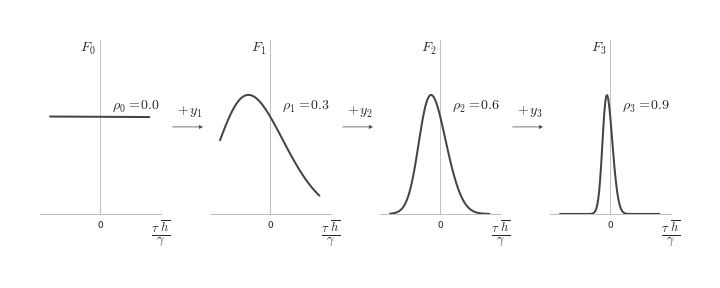
\includegraphics[scale=1.1]{modulation-function-rho.png}
\end{figure*}

\newcommand{\EF}{\ensuremath{\mathrm{F}(\,\htv\,|\gmt,\tau,\ns)}} O gradiente da função $\EV$ pode ser visto como uma \emph{força} que atua sobre $\wt$ na direção que aproxima o aluno do professor, composta pela direção $\tau\,\vec{x}$ e uma amplitude $F$. Chamaremos essa amplitude de \emph{Função de Modulação Bayesiana}, e para futuras referências
\begin{align}\label{eq:f-bayes}
    \EF & = - {\tau}\,\del{\htv} \EV = {\tau\gmt^2}\,\del{\htv}
    \ln\inbk{\ns-(1-2\ns)H\inpr{-\frac{\tau\htv}{\gmt}}} \notag \\ & =
    \frac{\gmt}{\sqrt{2\pi}}(1-2\ns)
    \frac{\exp\inbk{-\half\inpr{\frac{\htv}{\gmt}}^2}}{\ns + (1-2\ns)
      H\inpr{-\frac{\tau\htv}{\gmt}}}
\end{align}

É possível mostrar \footcite{Kinouchi1996,Vicente1998} que a grandeza $\gmt$ está relacionada com semelhança entre aluno e professor, dada por $\rho = \frac{\rl^T\wt}{||\rl||||\wt||}$, da seguinte forma
\begin{align}
    \gmt^2 & = \frac{1-\rho^2}{\rho^2}\label{eq:rho-def}
\end{align}
Essa relação facilita a compreensão da evolução de $\Ct$ ao longo do aprendizado, associando a adaptação na função de modulação diretamente ao desempenho do aluno condizente com os acertos relativos ao professor.
Tal adaptação da função de modulação pode ser descrita como um ajuste da relevância dada pelo aluno ao conteúdo dos exemplos de acordo com a experiência obtida até então.

Para compreender o que se passa, olhemos para a grandeza $\frac{\tau\htv}{\gmt}$.
O sinal de $\frac{\tau\htv}{\gmt}$ indica que o aluno classificou correta ou incorretamente o exemplo apresentado, enquanto seu valor absoluto indica o grau de \emph{surpresa/tédio} que o exemplo causa no aluno.
Essa interpretação vem do fato que $\tau=\pm 1$ e, portanto, $|\htv|$ indica quanta certeza o aluno tem em sua resposta, e portanto, um erro quando há muita certeza gera mais surpresa do que um acerto numa situação semelhante.  Ao longo do aprendizado, $\rho$ tende a aumentar, fazendo com que a função de modulação se adapte para dar mais relevância a exemplos que causem maiores surpresas.

A desconfiança do aluno sobre a classificação do professor, representada pela estimativa $\ns$ da probabilidade do professor estar errado, faz com que a função de modulação reduza a relevância de surpresas muito grandes, dando à função de modulação um caráter adaptativo.
Uma ilustração do comportamento da função de modulação em relação parâmetro $\rho$ e $\ns$ é dada pelas figuras \ref{fig:Frho} e \ref{fig:Fns}

\begin{figure*}[h!]\label{fig:Fns}
  \centering 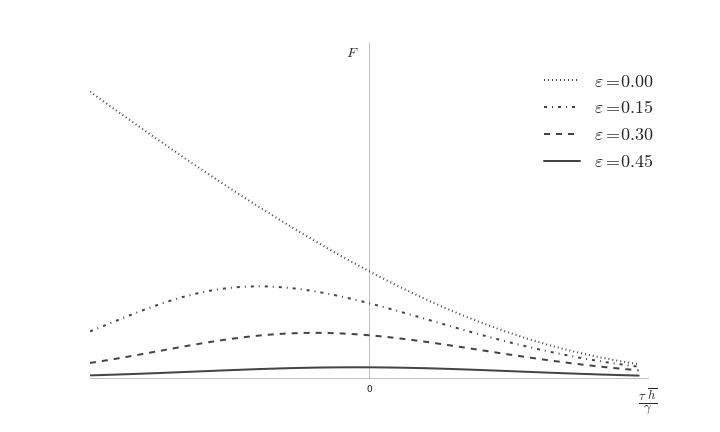
\includegraphics[scale=1.1]{modulation-function-eta.png}
  \caption{Comportamento da função de modulação $F$ com respeito ao aumento da desconfiança do aluno sobre possíveis erros do professor, para $\rho$ fixo. Valores de $\frac{\htv\tau}{\gmt}$ positivos ou negativos ocorrem quando o aluno classifica correta ou incorretamente o exemplo apresentado, o seu valor absoluto está associado com o grau de surpresa trazido pelo exemplo.}
\end{figure*}

Com base no cenário estabelecido, fica evidente que ao fixarmos um valor de $\rho$, fazendo com que a equação \eqref{eq:Ct-V} fique $\CT = \Ct$, a forma da função de modulação fica congelada.
Isso  é equivalente a fixar um algoritmo de aprendizado para o aluno que, na abordagem apresentada, é completamente determinado por $\rho$ e $\ns$.
A escolha de congelar a dinâmica para $\rho$, ao menos no que diz respeito à modelagem de comportamento humano, é motivada por estudos apontando que o desenvolvimento das áreas sociais do cérebro se desenvolvem no período da adolescência.
Nos estudos de \parencite{Choudhury2006, Blakemore2008,Moriguchi2007} é estabelecida, através de análises \emph{fMRI}, mudanças na atividade e na estrutura de áreas como o córtex pré-frontal, o córtex parietal e o córtex temporal superior, associados com o desenvolvimento da cognição social.
Neste trabalho, teremos sempre fixado um valor de $\rho$, sinalizando que a estratégia de aprendizado dos agentes foi previamente estabelecida, numa analogia com agentes \emph{``adultos''} do ponto de vista de cognição social.

A dedução acima foi feita com base na teoria de aprendizado de máquina e deixou de fora vários aspectos interessantes desse campo de estudo.
Leitores interessados no assunto podem consultar \parencite{Engel2001, Hastie1993} para abordagem completa e \parencite{Kinouchi1996, Solla1999,Opper1996} para aprofundar os conceitos apresentados nessa seção.

\subsection{Um Modelo mais Simples de Aprendizado}
\label{ssec:SLM}

A dedução acima nos proporciona um algoritmo de aprendizado supervisionado que maximiza o aprendizado por exemplo apresentado, mas essa vantagem é obtida pelo preço da interpretação do algoritmo, dificultada pela forma não muito amigável da função de modulação \eqref{eq:f-bayes}.
Para tentar sanar esse problema, vamos abstrair as características da função de modulação ótima e tentar criar uma forma mais simples que as mantenha.

Primeiramente, note que a equação \eqref{eq:f-bayes} como função da variável que mede $\frac{-\tau\,h}{\gmt}$ a concordância entre as respostas do aluno e do professor pode ser vista como uma atribuição de pesos para cada grau de concordância.
Em outras palavras, a função de modulação é responsável pela diferença na relevância dada a exemplos que corroboram a classificação do aluno e aqueles que o surpreendem, com $\frac{-\tau\,h}{\gmt}$ respectivamente positivos e negativos.
Essa é a principal característica dos algoritmos de aprendizado e, portanto, a principal forma de caracterizá-los.
Por exemplo, os algoritmos tradicionais como o de \emph{Hebb} ou o \emph{Perceptron} tem como única distinção o fato do primeiro dar mesmo valor a todos os exemplos e o segundo dar valor apenas aos que trazem novidade, que surpreendem.

No presente contexto, a forma de ajustar a relevância dada à exemplos com carga corroborativa ou surpreendente é fixando os valores do estilo cognitivo $\rho$ e da desconfiança $\ns$.
Podemos pensar uma forma simplificada, $F_{MF}$, para a função de modulação \eqref{eq:f-bayes} que tenha essas características de regular o peso entre corroboração e novidade através dos parâmetros $\rho$ e $\ns$.
Será útil também definir um custo cognitivo simplificado, $V_{MF}$, associado ao erro na classificação.

\newcommand{\EFmf}{\ensuremath{F_{MF}}}
\newcommand{\EVmf}{\ensuremath{V_{MF}}}
% A função de modulação \eqref{eq:f-bayes} é relativamente complicada, tornando impraticável o desenvolvimento analítico do modelos de mecânica estatística que serão desenvolvidos a seguir.
% Será útil, portanto, definir uma função de modulação mais tratável e que mantenha algumas das características descritas da equação \eqref{eq:f-bayes}.
% Em particular, vamos fazer com que a nova função que reproduza o comportamento da função de modulação relativo à diferença de relevância dada à exemplos corroborativos e novidades, bem como a possível regulação de absurdos.
% Através dessa nova função, que chamaremos $\EFmf$, podemos obter uma energia associada ao erro de classificação, à qual chamaremos $\EVmf$, definidos da seguinte forma
\begin{align}
    \EFmf(z|\,\rho,\ns,z_0) & = \frac{1-\rho}{2}
    - \frac{\rho}{2}\sgn(z)
    + \half\sgn(z+z_0) \label{eq:f-mf} \\[4pt]
    \EVmf(z|\,\rho,\ns,z_0) & = - \frac{1-\rho}{2}z
    + \frac{\rho}{2}|z| -
    \half|z+z_0| \label{eq:v-mf}
\end{align}
onde as grandezas $z$ e $z_0$ estão relacionadas com o parâmetro de concordância $\frac{-\tau\,h}{\gmt}$.

Para entender as grandezas $z$ e $z_0$, vamos olhar para o gráfico da funções \eqref{eq:f-mf}, ilustrado na figura \ref{fig:mf-func}, e associá-las às características descritas acima.
\begin{figure}[h!]\label{fig:mf-func}
    \centering
    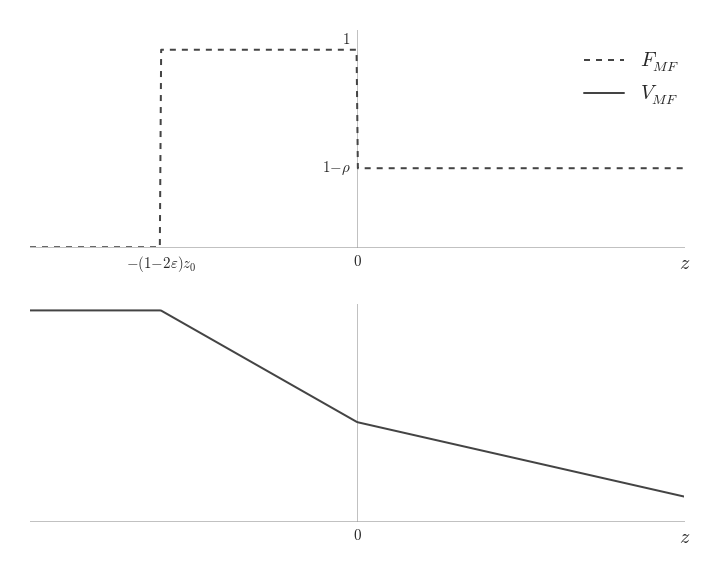
\includegraphics[scale=0.5]{mean-field.png}
    \caption{Ilustração das função aproximadas $\EFmf$ e $\EVmf$}
\end{figure}

Como discutido acima, $F_{MF}$ regula a relevância entre óbvio e novidade, logo $z$ deve ser uma função de $\frac{-\tau\,h}{\gmt}$.
O parâmetro $z_0$ é um valor de discordância que indica um conflito tão grande com o conhecimento do aluno que o faz ignorar a resposta do professor, ou seja é o ponto a partir do qual o aluno considera a informação daquele exemplo como \emph{'besteira'} e não o absorve.
É evidente, olhando para a função de modulação Bayesiana \eqref{eq:f-bayes}, que $z_0$ deve ser uma função de $\ns$ e $\rho$.

Para determinar o comportamento de $z_0$, basta otimizar o erro quadrático entre $F_{MF}$ e $F$ em relação ao valor de $z$, que levará ao valor $z=z_0$ para o qual $F$ tem a metade da altura máxima.
Alternativamente, é possível considerar $z_0$ como um grau de liberdade a mais no modelo e estudar sua influência no comportamento do campo médio.

% \vfill
\section{Modelos de Agentes e Mecânica Estatística}
\label{sec:AMSM}

\subsection{Estabelecendo a Linguagem do Modelo de Agentes}\label{ssec:AMSM1}
A hipótese central deste estudo de fenômenos sociais é que as propriedades de uma sociedade surgem da interação entre os indivíduos que a integram.
Essa forma de abordar o problema tem a vantagem de requerer apenas a compreensão do que é um indivíduo e como ele atua com outros semelhantes a ele, ou seja, é necessária apenas uma compreensão local do sistema para inferir algumas características globais.
É claro que essa estratégia pode ser criticada por um excesso de simplificação ao desconsiderar características particulares, tanto no que diz respeito ao indivíduo quanto a suas relações.
Entretanto, é necessário ter em mente que o objetivo não é detalhar o resultado de cada interação possível entre indivíduos, mas sim tentar reproduzir o comportamento macroscópico que observamos em diversas culturas e, se possível, sua relação com aspectos intrínsecos da natureza humana.

\newcommand{\agt}[1]{\ensuremath{\vec{w}_{#1}}}
\newcommand{\vrt}{\ensuremath{\mathcal{V}}}
\newcommand{\edg}{\ensuremath{\mathcal{E}}}
\newcommand{\MM}{\ensuremath{\mathcal{W}}}
Para elaborar um modelo de agentes capaz de descrever fenômenos sociais atribuídos a cultura, moral ou estratégias políticas, entre outros fenômenos relacionados a comportamento aprendido, precisamos entender ou, no mínimo emular, como se dá o processo de aprendizado social.
Considere um conjunto de vértices $\vrt = \{1,\dots,N\}$ e um conjunto de vetores $\MM = \{\agt{i} | i \in \vrt \}$, representando \emph{agentes} que interagem através da troca de informações e aprendem uns com os outros, de acordo com a estrutura das \emph{relações sociais} estabelecidas em $\edg \subset \vrt \times \vrt$ denotando $(ij)\in\edg$ quando os agentes $i$ e $j$ são parceiro sociais \footnote{Note que as relações estabelecidas em $\edg$ não são, necessariamente, simétricas.
É possível que um agente considere outro um parceiro sem   reciprocidade}.
Cada agente é representado por vetor $\agt{i} \in \R^K$ que representa sua experiência \footnote{num contexto determinado pelo fenômeno social em estudo} e um índice $i \in \vrt$, e pode receber a \emph{opinião} de um agente com quem se relaciona sobre um \emph{assunto} ou \emph{questão} $\vec{x} \in \R^K$ que tem alguma relação semântica com os vetores $\vec{w}$.

\newcommand{\cogcost}{\ensuremath{{\mathrm{V}}}}
\newcommand{\opn}[3][1]{\ensuremath{
      {#1\over \sqrt{K}} \agt{#2} \cdot \vec{#3}}}
\newcommand{\cost}{\ensuremath{{\mathcal{H}}}}
\newcommand{\SG}{\ensuremath{\mathcal{G}}}
\newcommand{\soc}{\ensuremath{\mathcal{S}}}
A interação entre dois agentes é regulada pelo custo cognitivo $\cogcost$, atribuído ao processo de aprendizado da \emph{opinião} $h = \opn{ }{x}$ de um agente pelo outro.
Considerando a soma do custo cognitivo sobre todos os pares de agentes no grafo temos o custo social total
\begin{align}
  \cost = \sum_{(i,j)\in \edg} J_{ij} \cogcost_{ij} \label{eq:Scost}
\end{align}
Chamaremos de \emph{Sociedade de Agentes}, ou apenas \emph{sociedade}, ao conjunto $\soc = (\SG, \MM, \cost)$, onde $\SG = (\vrt,\edg)$ é o grafo das interações sociais.

A natureza dos vetores $\MM$ depende do fenômenos em estudo.
No caso de aprendizado moral, como em \parencite{Cesar2014, Vicente2014}, o vetor $\agt{i}$ representa a matriz moral do agente $i$, e o processo de aprendizado entre os agentes pode levar ou não a um consenso sobre como é o comportamento \emph{ético} daquela sociedade.
Por outro lado, numa escala mais ampla, como no modelo em \parencite{Axelrod1997}, os vetores $\MM$ podem representar características culturais de agrupamentos de pessoas, cenário no qual cada agente representa, digamos, uma vila e a troca de características culturais entre agentes representa a dinâmica de estruturas culturais, possibilitando o surgimento de fronteiras isolando diferentes culturas que, de alguma forma, se tornaram \emph{incompatíveis}.

A topologia do grafo social, em particular o número de parceiros sociais, tem uma grande influência na possibilidade da sociedade experimentar uma transição de fases.
Somado a isso, o fato das estruturas sociais dependerem da dinâmica entre os indivíduos cria uma dinâmica para as relações entre agentes.
Esse efeito mútuo da influência do grafo nas características do indivíduo e vice-versa deve ser contemplado pelo modelo.
Para isso, introduzimos a matriz de adjacência das relações sociais, com elementos $R_{ij}$.
Estabeleceremos uma dinâmica para as relações sociais de modo que os valores de $R_{ij}$ estejam entre $0$ e $1$, se anulando quando os agentes $i$ e $j$ deixam de interagir, ou seja quando $(ij) \notin \soc$.
% \begin{equation}
%  R_{ij} =
%   \begin{cases}
%     0 < R \leq 1, & \text{ se } (ij) \in \edg \\
%     0, & \text{ caso contrário}
%   \end{cases}
% \end{equation}

A determinação da função custo cognitivo está relacionada com a dinâmica de aprendizado supervisionado desenvolvido na seção \ref{sec:ML} através de uma analogia. Cada agente na sociedade pode desempenhar tanto o papel de \emph{ aluno} quanto o de \emph{professor}.
Essa alternância de papeis é interpretada como uma sequência de diálogos entre agentes, nos quais ora um agente expressa sua opinião sobre uma questão, ora recebe a opinião de algum parceiro social.
Na situação em que a opinião de um colega é recebida, o agente se comporta como um aluno, tentando aprender a reproduzir o comportamento do outro agente. \footnote{É possível impor um comportamento antagonista, no qual um agente ativamente caminha no sentido oposto ao colega locutor.
A analogia se mantém considerando que o professor seria um agente com a orientação oposta à do agente que expressa a opinião.}

Com base nas equações \eqref{eq:wt-V}, \eqref{eq:Ct-V} e \eqref{eq:Vh}, podemos estabelecer um \emph{evento} envolvendo os parceiros sociais $(ij) \in \edg$ como uma relação \emph{aluno/professor} na qual $i$ aprende a opinião $h_j = \opn{j}{\vec{x}}$ do agente $j$ a respeito de um assunto $\vec{x}$.
O desempenho de $i$ com relação a essa tarefa é estimada pelo custo cognitivo $\cogcost_{ij}(\vec{x}) = V(\agt{i},\agt{j},\vec{x})$.

Como argumentado em \parencite{Cesar2014}, pessoas passam por diferentes estágios de aprendizado ao longo vida.
Quando mais  jovens, as estratégias de aprendizado social estão se formando, e podemos associar a resposta de uma criança ao se defrontar com diversos exemplos com a evolução da função de modulação ilustrada na figura \ref{fig:Frho}.
Ao passo que novidade é encontrada, a criança altera, de forma inconsciente, a relevância relativa dada a exemplos surpreendentes ou corroborativos.
Entretanto, após uma certa idade o modo como as pessoas aprendem fica \emph{`congelado`}, sendo associado a um algoritmo de aprendizado fixo no contexto de aprendizado de máquinas.
Em termos das equações da dinâmica de aprendizado \eqref{eq:wt-V} e \eqref{eq:Ct-V}, isso equivale à fazer $\gmt_i$ constante, e por consequência $\rho_i$ constante. Desse modo, fixando $\rho_i$, nossa analogia trata de agentes \emph{`adultos`} no aspecto de aprendizado social.
Com base nos argumentos dados em \parencite{Caticha2011}, a tendência de associação entre indivíduos mais parecidos nos estimula a fixar um único $\rho$ para grupos de agentes parceiros ou mesmo para toda uma sociedade.
\newcommand{\Vab}[2]{\ensuremath{\cogcost_{#1#2}}}
\newcommand{\gm}{\ensuremath{\gamma}}
\newcommand{\stb}{\ensuremath{\frac{\tau_j h_i}{\gm}}}
Com essas considerações, podemos escrever um custo cognitivo e a função de modulação para um evento entre os parceiros $i$ e $j$ da seguinte maneira
\begin{align}
    \Vab{i}{j}(\vec{x}) & = -\gm^2\ln\inbk{\ns
      + (1-2\ns)H\inpr{-\stb}} \label{eq:Vij}  \\[4pt]
    F_{ij}(\vec{x}) & = \frac{\gm(1 - 2\ns)}{\sqrt{2\pi}}
    \frac{\exp\inbk{-\half\inpr{\frac{h_i}{\gm}}^2}}{\ns
      + (1-2\ns)H\inpr{-\stb}} \label{eq:Fij}
\end{align}
onde $\tau_j = \sgn(h_j)$ e $\gm^2 = \frac{1-\rho^2}{\rho^2}$.

O parâmetro $\ns$, introduzido no contexto do aprendizado de máquina como uma estimativa do aluno para a probabilidade de receber uma informações equivocadas do professor, desempenha o papel de uma \emph{desconfiança} no contexto de aprendizado social, possibilitando a rejeição de opiniões muito dissonantes.
A interpretação da informação trazida por exemplos através de surpresa ou corroboração para o aluno no cenário do aprendizado de máquina é traduzido no contexto de aprendizado social para uma dicotomia entre \emph{concordância} e \emph{discordância} das opiniões.
Dessa forma, fica clara uma interpretação do custo cognitivo como um preço a ser pago pela discordância entre dois agentes e o custo social, $\cost$, como uma energia necessária para sustentar uma sociedade com um certo grau de diversidade nas opiniões dos agentes.

É evidente, pela forma do potencial $\Vab{i}{j}$, que embora opiniões \emph{`absurdas`} do agente $j$ sejam ignoradas pelo agente $i$, o mínimo global de $\cost$ estará mais próximo do estados de $\MM$ que desempenham o maior valor possível de concordância entre todos os agentes, caracterizando um consenso global quando o agentes trocam informação sobre uma questão apenas, como verificado em  \parencite{Caticha2011}.

Para sustentar a coexistência de diversidade entre agentes com as mesmas características cognitivas, a saber $\rho$ e $\ns$, é necessário criar um mecanismo que reduz o custo pago em presença de discordância, aliviando a pressão social.
Isso é feito dando a cada agente o poder de construir ou destruir suas relações sociais por meio das opiniões recebidas, através do controle das relações sociais $R_{ij}$.
A dinâmica das relações sociais é definida da seguinte forma
\begin{align}
  R_{ij}^{+} & = (1-\varphi)R_{ij} + \lambda R_{ij}(1 - R_{ij})\sgn(h_ih_j) \label{eq:Rt}
\end{align}
onde $R_{ij}^{+}$ é a relação entre $i$ e $j$ após um evento de interação, $\lambda$ um parâmetro que controla a \emph{`euforia`} no ajuste da relação e $\varphi$ um parâmetro que controla o \emph{`esquecimento`} dessa relação. A grandeza $J_{ij}=J(R_{ij})$ que aparece na equação \eqref{eq:Scost} está relacionada, de alguma forma a ser escolhida de acordo com o contexto específico do fenômeno estudado,com as relações sociais $R_{ij}$ e tornará possível a regulação do comportamento de aproximação ou rejeição relativo a uma opinião.
Note que as relações sociais se intensificam caso os agentes concordem num evento e são reduzidas caso contrário, fazendo o papel de uma espécie de registro da taxa de concordância do agente $i$ com as opiniões do agente $j$.

\subsection{Mecânica Estatística de Sistemas Sociais}\label{ssec:AMSM2}

Do que foi discutido na elaboração da linguagem que usaremos ao lidar com fenômenos sociais, ficam claros dois pontos importantes do modelo: sua natureza estatística e a importância delegada ao custo social, $\cost$.
Para avançar, faremos uso de métodos típicos da mecânica estatística, possibilitando a compreensão de alguns termos usado de forma vaga anteriormente, como \emph{`consenso`} ou \emph{`pressão`} e providenciando algumas previsões de comportamento do modelo.

Primeiramente, vamos determinar a probabilidade $P(\MM)$ de termos
uma sociedade $\soc = (\MM, \SG, \cost)$ num determinado estado $\MM$ com uma configuração social $\SG$ fixa.
Dos argumentos apresentados, somos levados a esperar algum valor para a função custo, ou seja devemos ter $P(\MM)$ tal que $\langle\cost\rangle=E \in \R$, onde $\langle\dots\rangle$ denota o valor esperado sobre $P(\MM)$.
Embora não tenhamos o valor $E$ para cada estado, essa expectativa indica nosso interesse na avaliação da função $\cost$.

A determinação de $P(\MM)$ é feita através da maximização da entropia relativa dela com alguma à priori $Q(\MM)$, que tomamos como uma distribuição uniforme em $\MM$ \footnote{Essa escolha é guiada pelo princípio da máxima ignorância e pelo fato da distribuição à priori carregar o mínimo de informação a respeito de um conjunto de variáveis, a saber apenas os possíveis valores que elas podem tomar.}, sujeita ao vínculo de valor esperado do custo social.
A entropia relativa entre $P$ e $Q$ é dada por
\begin{align}\label{eq:ent-Pw}
  S[P(\MM):Q(\MM)] & = -\int \msr{\MM} P(\MM) \ln \frac{P(\MM)}{Q(\MM)} \notag \\
                   & \quad + \beta \inbk{E - \int \msr{\MM} P(\MM)\cost}
\end{align}

Igualando a zero derivada funcional de $S$ relativa a $P$, notando que $Q$ é uma constante, obtemos a forma da distribuição $P$ que maximiza a entropia, a saber a distribuição de \emph{Boltzmann}, dada por
\begin{align}
  P(\MM) & = \frac{1}{Z} \exp (-\beta \cost [\MM]) \label{eq:Pw} \\
\intertext{onde $Z$ é a função de partição}
  Z & = \int \msr{\MM} \exp (-\beta \cost [\MM]) \label{eq:Zw}
\end{align}

O parâmetro $\beta$, introduzido como um multiplicador de \emph{Lagrange} associado ao vínculo do valor esperado do custo social, pode ser interpretado analisando a distribuição $P$ obtida.
Note que, supondo um valor fixo de $\beta \neq 0$, estados com custos sociais mais elevados se tornam menos prováveis de acordo com $P(\MM)$.
Isso implica que a evolução da sociedade sobre a dinâmica definida por $\cost$ deve seguir na direção de reduzir os custos sociais. Neste caso, $\beta$ é uma espécie de \emph{pressão}, determinando a escala de flutuações do custo social relativo ao valor esperado $E$.

A natureza da pressão $\beta$ depende em parte do contexto, embora seja claro que ela está relacionada com a pressão sobre cada agente perante a exibição de um comportamento \emph{`transgressor`} relativo a seus parceiros, e por esse motivo a chamaremos de \emph{pressão social} \footnote{No contexto de concorrência partidária, daremos um nome mais sugestivo para a pressão, mas por enquanto, pressão social é suficiente para o entendimento do que segue.}.
Essa interpretação nos leva a crer que, fixadas as relações sociais, ou seja fazendo $R_{ij}$ constantes, e dada suficiente pressão encontraremos a sociedade apenas em estados de \emph{consenso} de opinião a respeito da questão colocada.
Para testar essa intuição, seguiremos com um estudo de campo médio visando estabelecer as condições em que tal situação de consenso pode ocorrer.

\newcommand{\qst}{\ensuremath{\vec{x}}}
\newcommand{\cutoff}{\ensuremath{\eta}}
Considere uma sociedade $\soc_0=(\MM,\SG,\cost_0)$, com as relações sociais $\SG$ fixadas a função custo social $\cost_0 = \sum J_{ij} V^0_{ij}$ com
\begin{align}\label{eq:V0ij}
  V^0_{ij} & = -\frac{1-\rho}{2}h_ih_j +\frac{\rho}{2}|h_ih_j|
               - \half|h_ih_j + \cutoff|
\end{align}
uma aproximação do custo cognitivo, como destacado na seção \ref{sec:ML} com a equação \eqref{eq:v-mf}. Os agentes são descritos por vetores $\agt{i}\in\R^K$ e trocam opiniões sobre um único assunto $\qst\in\R^K$.
Vamos supor que $|\agt{i}|^2=|\qst|^2=K$ para todo $i$ e chamar $h_i = \opn{i}{\qst}$, de modo que $-\sqrt{K} \leq h_i \leq \sqrt{K}$ e $\cutoff = (1-2\ns)K$.
Essa escolha para o valor de $\cutoff$ está relacionada com o parâmetro $z_0$ comentado na seção \ref{ssec:SLM}, tratando-o como um grau de liberdade extra, e pode ser encarada como um modelo para o comportamento de $\cutoff$ em termos de $\ns$.
Como veremos, a influência de $\cutoff$ para um valor linear em $\ns$ não afeta as fases observadas no campo médio, dissonando do resultado obtido para o potencial Bayesiano.

Para possibilitar o tratamento da função de partição \eqref{eq:Zw}, além da introdução do potencial $V^0$, vamos supor que os $J$ são distribuídos de forma homogênea em $\SG$, ou seja
\begin{equation*}
  J_{ij} = \begin{cases}
    J_0 > 0 & \text{se $i$ e $j$ são parceiros sociais} \\
    0 & \text{caso contrário}
    \end{cases}
\end{equation*}
e que $\SG$ é um grafo regular não direcionado, o que significa que cada agente tem o mesmo número $n_0$ de parceiros e todas as relações são recíprocas.
\footnote[][-7cm]{Essa hipótese é bem restritiva, mas não é artificial, dado que grafos sociais frequentemente apresentam uma estrutura quase regular como grafos de \emph{mundo pequeno}, onde o grau médio de cada vértice é representativo globalmente.
Esse pode não ser o caso em estruturas mais assimétricas como  grafos de \emph{Barabasi-Albert}.
Mas em se tratando do campo médio, a estrutura do grafo seria descartada de todo modo, então essas consideração servem apenas para indicar as situações em que os resultados simulados ou experimentais não podem ser explicado apenas pela aproximação de campo médio.}

Com essas hipóteses adicionais, podemos nos questionar qual é a distribuição $P_* = \prod_i^N P_i$, sujeita ao vínculo do valor esperado do custo social, que melhor aproxima a distribuição $P(\MM)$ por um sistema de agentes independentes?
Para responder essa pergunta, usamos mais uma vez a maximização da entropia em relação às distribuições $P_i$.
A entropia relativa entre $P$ e $P_*$ é
\begin{align}
  S[P_*:P] & = -\int \msr{\MM} P_* \ln \frac{P_*}{P}
               + \beta\inbk{E - \int\msr{\MM}P_*\cost} \notag\\
           & = -\sum_j^N\int\msr{\agt{j}}P_j\ln {P_j \over P}
               \notag\\
           & \quad + \beta\inbk{E-\sum_{(kj)\in\SG}\int
                 \msr{\agt{k}}\msr{\agt{j}}P_kP_jJ_0V^0_{kj}}
               \label{eq:ent-P*}
\end{align}
onde usamos implicitamente a normalização de cada $P_j$.
Tomando a derivada funcional de S em relação a $P_i$ e igualando a zero teremos, usando o fato de $P$ e $E$ serem independentes de $P_i$
\begin{align}
   0 = {\delta S \over \delta P_i} & = 1 - \ln P_i -\beta J_0\sum_{j\in n(i)}\int\msr{\agt{j}}P_jV^0_{ij} \notag\\
  \Rightarrow P_i & = \frac{1}{Z_i}\exp\inbk{-\beta J_0 \sum_{j\in n(i)}\int \msr{\agt{j}}P_j V^0{ij}} \label{eq:PiV}
\end{align}
denotando por $n(i) = \{j | (ij)\in \SG \}$ o conjunto dos parceiros sociais do agente $i$.

Para prosseguir, será necessário trabalhar com a integral
\begin{align}
  I_i & = \int \msr{\agt{j}}P_j V^0_{ij} \notag\\
      & = \int \msr{\agt{j}}P_j \inbk{-h_ih_j + \frac{\rho}{2}|h_ih_j| - \half|h_ih_j+\cutoff|} \label{eq:lnPiV}
\end{align}
que aparece no lado direito da equação \eqref{eq:PiV}.
Somente nesse ponto a escolha do custo cognitivo \eqref{eq:V0ij} se justifica, tendo em vista que mesmo a definição dos parâmetros de ordem, no que seguirá, seria mais difícil, senão impossível, com o potencial \eqref{eq:Vij}.
Note também que, o potencial \eqref{eq:V0ij} é uma forma um pouco mais geral daquele usado em \parencite{Caticha2011}, se reduzindo àquele no caso em que a desconfiança é nula, ou seja $\ns = 0$.
De fato, a análise de campo médio apresentada aqui segue os moldes da estabelecida em \parencite{Caticha2011,Cesar2014}.

Para determinar a distribuição $P_i$, definimos os parâmetros de ordem
\begin{align}
  m & = \int \msr{\agt{j}} P_j \opn{j}{\qst} \label{eq:m-def} \\
  r & = \int \msr{\agt{j}} P_j \left|\opn{j}{\qst}\right| \label{eq:r-def}\\
\intertext{e substitua em \eqref{eq:lnPiV} para obter}
  I_i & = -m{1-\rho \over 2 \sqrt{K}}\agt{i}\cdot\qst
          +r\,\frac{\rho}{2\sqrt{K}}\left|\agt{i}\cdot\qst\right|
          - {1\over 2 \sqrt{K}}\left|m\,\agt{i}\cdot\qst+\cutoff\right| \label{eq:Ii}
\end{align}
Note que assumimos a homogeneidade dos parâmetros de ordem, ou seja, fizemos $m_j = m$ e $r_j = r$ para todo $j$.
Isso não  significa que os são idênticos, mas que são descritos de forma idêntica.
Essa hipótese está relacionada com a homogeneidade das relações, explicitada pela constante $J_0$.
Fizemos também a escolha de comutar a integral com o valor absoluto no termo que envolve a desconfiança para facilitar as contas e por manter a coerência, mas sem uma justificativa formal para isso.
Substituindo \eqref{eq:Ii} em \eqref{eq:PiV} e lembrando que todos agentes têm o mesmo número de parceiros $n_0$, chegamos à conclusão
\begin{align}
  P_i & = \frac{1}{Z_i}\EulerE^{-\beta\,J_0\,n_0\,I_i} \label{eq:Piw}
\end{align}

O resultado obtido para as probabilidade $P_i$ nos traz um conjunto de equações que precisam ser resolvidas de forma autoconsciente, a saber
\begin{align}
  m & = \frac{1}{Z} \int \msr{\agt{i}} \inpr{\opn{i}{\qst}}\EulerE^{-\beta\,J_0\,n_0\,I_i(m,r)} \label{eq:sc-m}\\
  r & = \frac{1}{Z} \int \msr{\agt{i}} \left|\opn{i}{\qst}\right|\EulerE^{-\beta\,J_0\,n_0\,I_i(m,r)} \label{eq:sc-r}\\
  Z & = \int \msr{\agt{i}}\EulerE^{-\beta\,J_0\,n_0\,I_i(m,r)} \label{eq:sc-Z}
\end{align}
A solução desse sistema de equações resulta na determinação das distribuições $P_i$ para todo os agentes, e por consequência determina nossa aproximação de campo médio.
Entretanto, a equação \eqref{eq:Piw} nos dá a probabilidade $P_i = P(\agt{i})$ de encontrar um agente com um estado interno $\agt{i}$ do agente.
Essa situação é inconveniente por dois motivos, a saber, por não termos acesso direto ao estado cognitivo das pessoas nos processos formadores de opinião e, também, por estarmos interessados, de fato, nas opiniões.
Para resolver esse conflito entre o resultado \eqref{eq:Piw} e sua praticidade, façamos
\begin{align}
  P(h) & = \int \msr{\agt{ }} \delta\inpr{h - \opn{ }{\qst}} P(\agt{ }) \notag \\[4pt]
       & = \frac{1}{C}(1 - h^2)\,\EulerE^{\,\beta J_0 n_0 \inbk {
         \frac{1-\rho}{2}hm - \frac{\rho}{2}|h|r + \half|hr + \cutoff|}} \label{eq:Ph}\\
\intertext{com a nova função de partição $C$ dada por}
  C & = \int _{-\sqrt{K}}^{\sqrt{K}} \msr{t} (1 - t^2)\,\EulerE^{\,\beta J_0 n_0\inbk{
       \frac{1-\rho}{2} mt - \frac{\rho}{2}r|t| + \half|rt + \cutoff|}} \label{eq:Zh}
\end{align}

Os parâmetros ordem $m$ e $r$ são os valores esperados das opiniões e das suas \emph{`convicções`} sobre $\qst$ em toda a sociedade.
Com isso podemos estudar as condições definidas pela pressão social $\beta$, pelo estilo cognitivo $\rho$ e pela desconfiança $\ns$ na formação de consenso através dos valores dos parâmetros de ordem. O comportamento típico do parâmetro $m$, que mede a média das opiniões em relação à questão dada, está ilustrado na figura \ref{fig:pd-ferro}.

\begin{figure}[h!]\label{fig:pd-ferro}
  \centering
  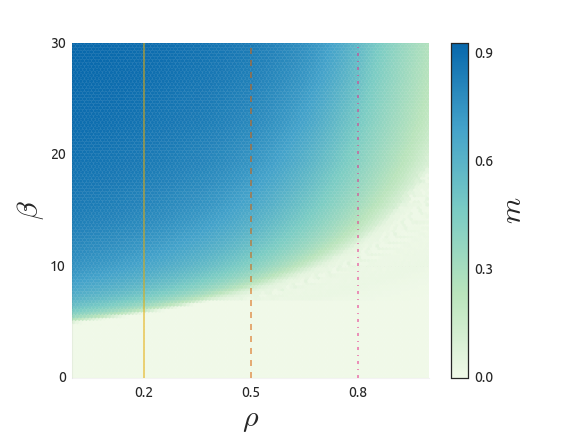
\includegraphics[scale=1.0]{phase-diagram-ferro.png}
  \caption{Diagrama de fases da solução $m$ das equações de campo médio, no plano $\beta \times \rho$.
Esse comportamento não se altera para baixos valores da desconfiança $\ns$ neste cenário de agentes similares em estratégia de aprendizado e motivados a cooperar.}
\end{figure}
\begin{marginfigure}[-7cm]
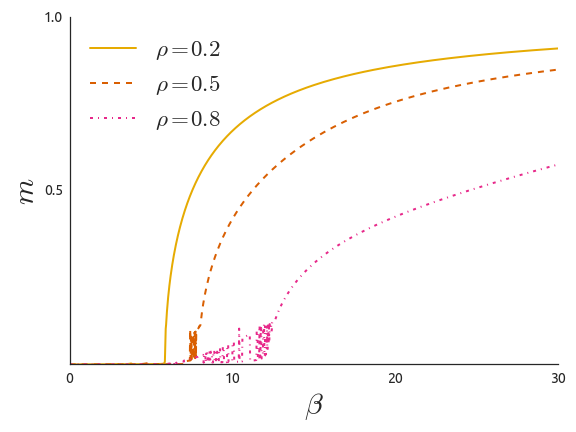
\includegraphics[scale=1.5]{m-curves-ferro.png}
\caption{Curvas de consenso correspondentes às retas verticais na figura \ref{fig:pd-ferro}.}
\end{marginfigure}

A figura \ref{fig:pd-ferro} mostra que, seguindo uma das linhas verticais que fixa um valor de $\rho$, há uma transição de fase entre os estados de dissenso e consenso com relação às opiniões dos agentes a respeito da questão $\qst$.
Sem se desprender do contexto, no cenário em que a concordância é estimulada, dado o parâmetro $J_0 > 0$, existirá uma pressão social crítica que levará essa sociedade ao consenso.
Esse tipo de comportamento é que esperamos dentro de um grupo com alguma ideologia ou de agentes que compartilhem um certo conjunto de características não muito disperso, codificado nos vetores $\agt{i}$.
Analogamente, situações onde a concordância seja muito relevante, talvez em condições de perigo à sociedade, é de se esperar que a sociedade atinja o consenso em detrimento da manutenção de diferenças.

Note, porém que maiores valores de $\rho$ tendem a apresentar pressões críticas mais elevadas.
Podemos imaginar numa sociedade com diferentes valores de $\rho$ a possibilidade de parte dos agentes estarem sob suficiente pressão social para obter consenso, mas outra parte não.
Logo, a analogia com ameças à sociedade nos levaria a associar essa variação às diferenças no que os agentes consideram ameaça ou não.
Essa aparente dicotomia sugere uma relação entre os comportamentos liberal e conservador exibido pelas pessoas e uma análise mais detalhada dessa relação pode ser encontrada em \parencite{Caticha2011,Vicente2014,Cesar2014}.

\begin{figure}[t!]\label{fig:pd-ferro-eps}
  \centering
  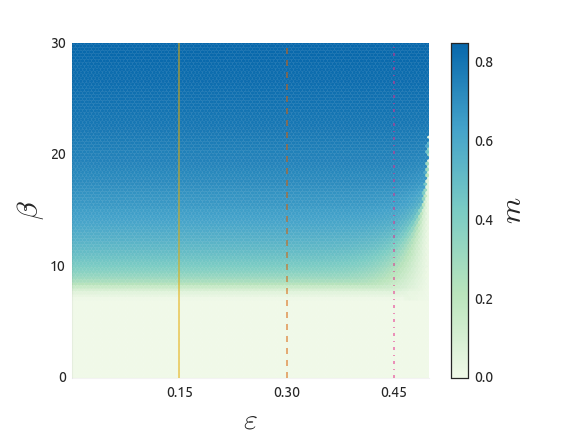
\includegraphics[scale=1.0]{eps-phase-diagram-ferro.png}
  \caption{Diagrama de fases da solução $m$ das equações de campo médio, no plano $\beta \times \varepsilon$.
Note como apenas valores de $\ns$ próximos de $0.5$ introduzem dificuldades ao surgimento de consenso.
Isso significa que, em campo médio, apenas sociedade em que quase nenhuma confiança pode ser atribuída aos parceiros é possível impedir o consenso.}
\end{figure}
\begin{marginfigure}[-9cm]
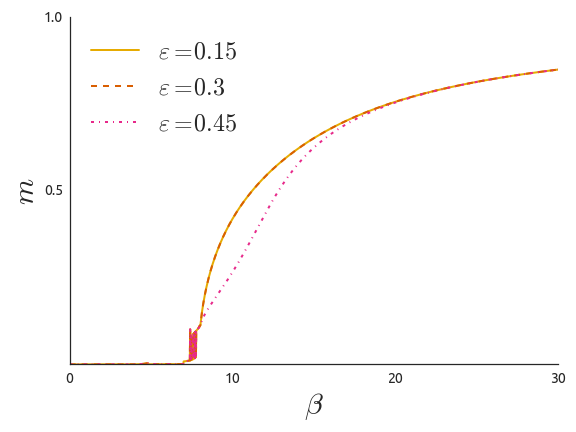
\includegraphics[scale=1.5]{eps-m-curves-ferro.png}
\caption{Curvas de consenso correspondentes às retas verticais na figura \ref{fig:pd-ferro-eps}.}
\end{marginfigure}

Uma propriedade interessante desse resultado é sua robustez perante mudanças na desconfiança $\ns$, como pode ser visto na figura \ref{fig:pd-ferro-eps}.
Essa condição nos diz relações internas de algum segmento social tendem a atingir consenso, mesmo com pouca confiança nas opiniões dos parceiros.
Tendo em vista a diversidade de opiniões relativas a um dado assunto, essa conclusão é de fato irreal.
O caso é que fixadas as relações sociais, a pressão dos pares eventualmente conduz ao consenso numa \emph{`vitória`} por resistência.

Vejamos um cenário em que uma sociedade tem dois grupos \emph{`rivais`} coexistindo.
Nessa situação, cada agente $i$ pode integrar um grupo $A=\{1,\dots,N_A\}$ ou um grupo $B=\{1,\dots,N_B\}$.
O custo cognitivo da interação entre os quaisquer dois agentes $(ij)$ é dado pela equação \eqref{eq:V0ij}, porem as grandezas $J_{ij}$ que regulam as interações sociais dependem dos grupo de $i$ e $j$.
Considere
\begin{align}\label{eq:J-antiferro}
  J_{ij} =
  \begin{cases}
    1 & \text{se $i$ e $j$ estão no mesmo grupo} \\
    -J & \text{com $J > 0$ caso contrário}
  \end{cases}
\end{align}
de modo que o custo social pode ser escrito
\begin{align}
  \cost_{AB} & = \sum_{\substack{i\in A\\j \in A}} V^0_{ij}
  + \sum_{\substack{i\in B\\j \in B}} V^0_{ij}
  - J\sum_{\substack{i\in A\\j \in B}} V^0_{ij} \label{eq:H-antiferro}
\end{align}
e podemos aplicar uma aproximação de campo médio análoga à feita para o cenário anterior.

Vamos aproximar a distribuição de \emph{Boltzmann} para a sociedade com custo social $\cost_{AB}$ por uma distribuição $P_{AB}=\prod_{i\in A}P_A(\agt{i})\prod_{j\in B}P_B(\agt{j})$, novamente através da maximização da entropia.
Seguindo essa estratégia, obteremos as seguinte formas para $P_A(\agt{i})$ e $P_B(\agt{j})$
\begin{align}
  P_A(\agt{i}) & \propto \EulerE^ {-\beta I_A(\agt{i})} \label{eq:PA}\\
  P_B(\agt{j}) & \propto \EulerE^ {-\beta I_B(\agt{j})} \label{eq:PB} \\
\intertext{com os termos $I_A$ e $I_B$ dados por}
  I_A(h_i) & = \sum_{k\in A}\int \msr{\agt{k}} P_A(\agt{k}) V^0_{ik}
  - J \sum_{l\in B} \int \msr{\agt{l}} P_B(\agt{l}) V^0_{il}
  \label{eq:IA} \\
  I_B(h_j) & = \sum_{l\in B}\int \msr{\agt{l}} P_B(\agt{k}) V^0_{jl}
  - J \sum_{k\in A} \int \msr{\agt{k}} P_A(\agt{k}) V^0_{jk}
  \label{eq:IB}
\end{align}
e para lidar com as integrais que aparecem em $I_A$ e $I_B$, definimos as seguintes grandezas
\begin{align}
  m_A & = {1\over Z_A}\int\msr{\agt{k}}\EulerE^{-\beta I_A(\agt{k})}\opn{k}{\qst} \\
  r_A & = {1\over Z_A}\int\msr{\agt{k}}\EulerE^{-\beta I_A(\agt{k})}\left|\opn{k}{\qst}\right| \\
  Z_A & = \int\msr{\agt{k}}\EulerE^{-\beta I_A(\agt{k})} \\
\intertext{para o grupo $A$ e analogamente para o grupo $B$}
  m_B & = {1\over Z_B}\int\msr{\agt{l}}\EulerE^{-\beta I_B(\agt{l})}\opn{l}{\qst} \\
  r_B & = {1\over Z_B}\int\msr{\agt{l}}\EulerE^{-\beta I_B(\agt{l})}\left|\opn{l}{\qst}\right| \\
  Z_B & = \int\msr{\agt{l}}\EulerE^{-\beta I_B(\agt{l})}
\end{align}
que definem um conjunto de equações auto consistentes que  determinam as probabilidades $P_A$ e $P_B$.

Usando o mesmo truque da equação \eqref{eq:Ph} obtemos as distribuições de opinião dos grupos $A$ e $B$, a menos da determinação das equações acima, a saber
\begin{align}
  P_A(h) & = {1\over Z_A}(1-h^2)\,\EulerE^{-\beta U_A(h)} \\
  P_B(h) & = {1\over Z_B}(1-h^2)\,\EulerE^{-\beta U_B(h)} \\
\intertext{com as funções de partição}
  Z_A & = \int_{-\sqrt{K}}^{\sqrt{K}}\msr{t}(1-t^2)\,\EulerE^{-\beta U_A(t)} \\
  Z_B & = \int_{-\sqrt{K}}^{\sqrt{K}}\msr{t}(1-t^2)\,\EulerE^{-\beta U_B(t)} \\
\intertext{e os logaritmos $U_A$ e $U_B$ dados por}
  U_A(h) & = -{1-\rho\over2}(N_Am_A - JN_Bm_B)h \notag\\
  & + {\rho\over2}(N_Ar_A-JN_Br_B)|h| \notag \\
  & - \half(N_A|m_Ah+\cutoff|-JN_B|m_Bh+\cutoff|) \\
  U_B(h) & = -{1-\rho\over2}(N_Bm_B - JN_Am_A)h \notag\\
  & + {\rho\over2}(N_Br_B-JN_Ar_A)|h| \notag \\
  & - \half(N_B|m_Bh+\cutoff|-JN_A|m_Ah+\cutoff|)
\end{align}

A solução desse conjunto de equações auto consistentes nos leva à distribuição de opiniões no caso em que dois grupos antagônicos coexistem sem uma relação de dominância ou estrutura hierárquica entre eles, em outras palavras numa situação de pluralidade de opiniões.
Para medir essa pluralidade, olhamos para o parâmetro de ordem \emph{`antiferromagnético`} $$m_s = {m_A - m_B \over 2}\text{,}$$ que se anula quando os grupos $A$ e $B$ compartilham da mesma opinião e tem valores mais próximos de $\pm 1$ de acordo com o quão opostas suas opiniões são.
O comportamento dessa sociedade simples é ilustrado na figura \ref{fig:pd-antiferro}

\begin{figure}[h!]\label{fig:pd-antiferro}
  \centering
  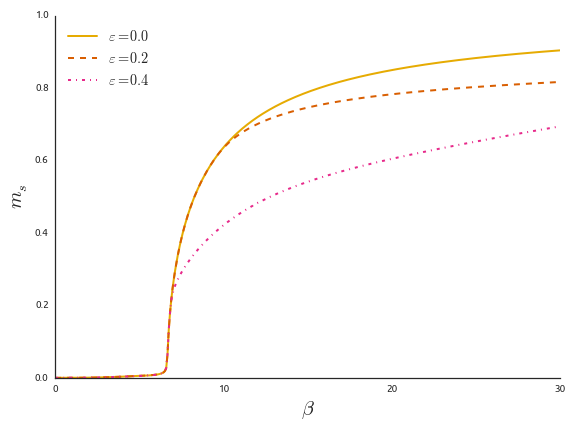
\includegraphics[scale=1.0]{phase-diagram-antiferro.png}
  \caption{Curvas da pluralidade de opiniões $m_s$ em função da pressão $\beta$ para diferentes valores da desconfiança $\ns$ e valor fixo do algorítimo de aprendizado $\rho=0.5$.
Note que conforme a desconfiança aumenta, o valor absoluto de $m_s$ cai, comportamento que se repete em $m_A$ e $m_B$, indicando a dificuldade na formação das opiniões intragrupo em situações de desconfiança.}
\end{figure}

Note que o aumento da desconfiança influencia a convicção de cada grupo em sua própria opinião, de modo que $m_s$ apresenta valores menores conforme a desconfiança $\ns$ aumenta.
Isso nos indica que a desconfiança associada às relações sociais pode ser um mecanismo que possibilita a diversidade de opiniões numa sociedade.

Para explorar essa nova possibilidade, investigaremos no capítulo \ref{ch:C3} dinâmicas para a formação de grupos dentro de uma sociedade e outros cenários em que a coexistência de grupos leva a comportamentos de interesse em eventos reais.


%% Capítulo 3

%%% Capítulo 3 - Aspectos Matemáticos

\chapter{Experimentos Computacionais e Análise dos Resultados}
\label{ch:C3}
% \chapquote{
% }{}

Apesar do esforço no sentido de simplificar ao máximo durante a elaboração do modelo para abordar relações sociais, a complexidade das equações da dinâmica não permitem um tratamento analítico além do desenvolvido no capítulo \ref{ch:C2} com as soluções de campo médio em condições bem restritivas.
Para explorar melhor as capacidades do modelo passamos agora a uma análise computacional da termodinâmica resultante da evolução de uma sociedade sob certas condições.

Para isso, começaremos descrevendo brevemente os métodos utilizados, sem detalhes de implementação, e seguiremos com a construção de cenários e a análise dos resultados neles obtidos.
O tratamento apresentado neste capítulo supõe familiaridade com o algoritmo de \emph{Metropolis} em Monte Carlo e com a termodinâmica de modelos magnéticos, como o de Ising.

\section{Monte Carlo em Sociedades de Agentes\\e a Termodinâmica de Consenso}
\label{sec:MCCT}

Para elaborar uma dinâmica de Monte Carlo para um sistema de agentes, vamos nos basear na forma como as relações ocorrem no cotidiano.
Podemos imaginar um cenário em que duas pessoas se encontram, expõem suas opiniões, possivelmente aprendem algo e seguem suas vidas.
Um passo \emph{`microscópico`} do algoritmo deve seguir esse roteiro, visando ser minimamente realista.

Para tentar formalizar essa sequência de eventos, consideremos $\soc$ uma sociedade com agentes $\MM$ em $\R^K$, $\SG$ um grafo completo e custo cognitivo
\begin{align}
\cogcost_{ij} & =-\gm^2\ln\inbk{\ns+(1-2\ns)H\inpr{-\frac{\tau_j\,h_i}{\gm}}} \tag{\ref{eq:Vij}}
\end{align}
O encontro de dois agentes, num passo microscópico $t$, é emulado sorteando um agente $i$ de maneira uniforme em $\soc$ e, em seguida, sorteando um de seus parceiros $j$ com probabilidade $p(j|i)$.
A conversa entre os agentes $i$  e $j$ pode resultar numa mudança no vetor cognitivo $\agt{i}(t)$, que ocorre através da proposta de um novo vetor $\vec{v} \in \R^K$.
A proposta é aceita com base na diferença do custo social entre o vetor proposto e o estado atual do agente $i$.
De maneira mais precisa, a probabilidade da proposta ser aceita é dada por
\begin{align}
  p(\agt{i}(t)\to\vec{v}) & =\min\inpr{1, \EulerE^{-\beta\,J_{ij}\Delta \cogcost}}\text{,} \label{eq:Pacc}
\end{align}
com $\Delta \cogcost = \cogcost(\vec{v},\agt{j}) - \cogcost(\agt{i}(t),\agt{j})$, de modo que $\agt{i}(t+1) = \vec{v}$ com probabilidade $p(\agt{i}(t)\to\vec{v})$.
O termo $J_{ij}$ pode depender da relação $R_{ij}$ entre os agentes, mas vamos mantê-lo constante $J_{ij}=\frac{1}{K}$, por enquanto, para estudar o cenário de formação de consenso.
Ao longo da simulação foi mantido o vínculo de normalização sobre os agentes, de forma que $|\agt{i}(t)|^2=K$ para todo $t \in \{1,\dots,T\}$ e todo $i \in \soc$, assim como sobre a questão $|\qst|^2=K$.
Além disso, a cada parceiro $j$ do agente $i$ foi dada a mesma probabilidade de ser escolhido, ou seja
\begin{align}
p(j|i) & = \frac{R_{ij}}{\sum_{k}R_{ik}} \label{eq:P(j|i)}
\end{align}
com $R_{ij}$ constantes, neste cenário, e dados por
\begin{align}
R_{ij} & = \begin{cases}
  1, & \text{ se } i \neq j \\
  0, & \text{ se } i = j
\end{cases} \label{eq:Rij-consensus}
\end{align}

Essa dinâmica de interação entre os agentes é repetida um número $T = MN$ de vezes, onde $N$ é o número de agentes em $\soc$ e $M$ é o número médio de vezes que cada agente é escolhido para aprender com um parceiro.
Em outras palavras, $M$ é o número de passos \emph{`macroscópicos`}, ou número de passos de Monte Carlo.
Em cada passo macroscópico, são medidas a média das opiniões e seus valores absolutos e suas respectivas correlações
\begin{align}
  m & = \frac{1}{N\sqrt{K}}\sum_{i=1}^N h_i \label{eq:def-m}\\
  r & = \frac{1}{N\sqrt{K}}\sum_{i=1}^N |h_i| \label{eq:def-r}\\
  q & = \frac{1}{N^2K} \sum_{(ij)}R_{ij} h_i h_j \label{eq:def-q}
\end{align}
além de outras grandezas relacionadas ao desempenho do Monte Carlo, como as taxas de aceitação.
Para mais detalhes sobre o método de Monte Carlo, recomendamos ao leitor o texto de \parencite{Newman1999}.

\subsection{As Fases de Uma Sociedade}

Os resultados das simulações dessa sociedade nos dizem quais a condições de pressão social $\beta$, estilo de aprendizado $\rho$ e desconfiança $\ns$ nas quais consenso podem surgir.
O diagrama de fases na figura \ref{fig:mc-pd-rho} mostra as fases de consenso numa sociedade com desconfiança $\ns=0$.
Como visto na discussão do capítulo \ref{ch:C2}, existe uma linha de transição entre as fases de desordem e consenso na sociedade e, ao menos qualitativamente, os resultados nas figuras \ref{fig:pd-ferro} e \ref{fig:mc-pd-rho} são equivalentes.

\begin{figure}[t!]\label{fig:mc-pd-rho}
    \centering
    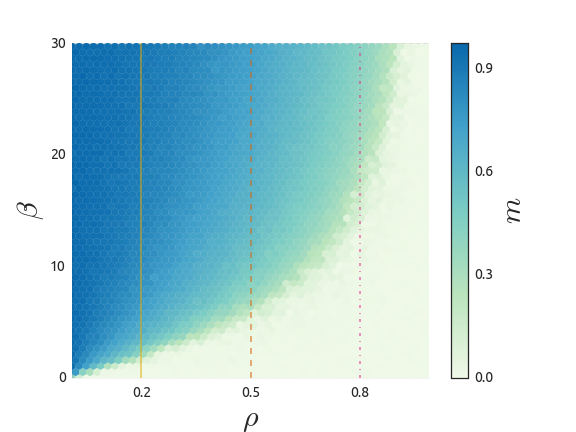
\includegraphics[scale=1.0]{mc-phase-diagram.png}
    \caption{Diagrama de fases do consenso $m$  no plano $\beta \times \rho$, para desconfiança $\ns = 0$.}
\end{figure}
\begin{marginfigure}[-11cm]
    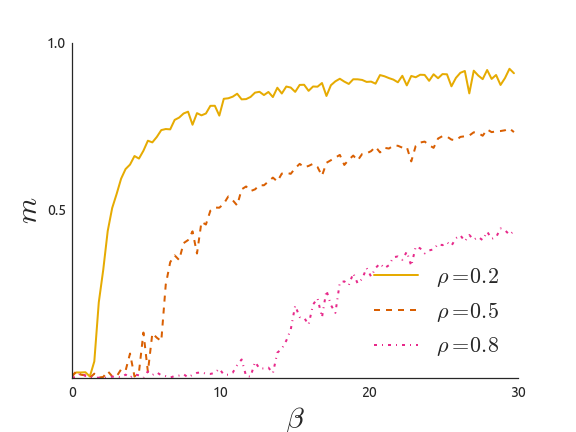
\includegraphics[scale=1.5]{mc-m-curves.png}
    \caption{Curvas de consenso correspondentes às retas verticais na figura \ref{fig:mc-pd-rho}.}
\end{marginfigure}


A diferença que surge na forma da fronteira que delimita as regiões vem do fato que o algoritmo de aprendizado definido por \eqref{eq:Vij}, a saber a função de modulação Bayesiana, é muito mais eficiente do que aquele oriundo da aproximação de campo médio \eqref{eq:V0ij}.
Por diferença na eficiência de um algoritmo de aprendizado entende-se que um número menor de exemplos precisa ser apresentado ao aluno para que ele aprenda a regra do professor.
No contexto de aprendizado social, isso significa que dois parceiros precisam interagir um número menor de vezes para que cheguem a uma opinião comum, e isso se reflete numa pressão crítica menor para que a sociedade atinja o consenso.
Essa é a exata diferença entre as figuras \ref{fig:pd-ferro} e \ref{fig:mc-pd-rho}.

Outra diferença que observamos entre os resultados da simulação de Monte Carlo e o resultado do campo médio é a dependência da pressão crítica com relação ao parâmetro de desconfiança $\ns$.
De fato, na simulação de Monte Carlo, o papel da desconfiança no surgimento de consenso é similar ao estilo cognitivo $\rho$, dificultando o consenso conforme seu valor aumenta.
\begin{figure}[h!]\label{fig:mc-pd-eps}
    \centering    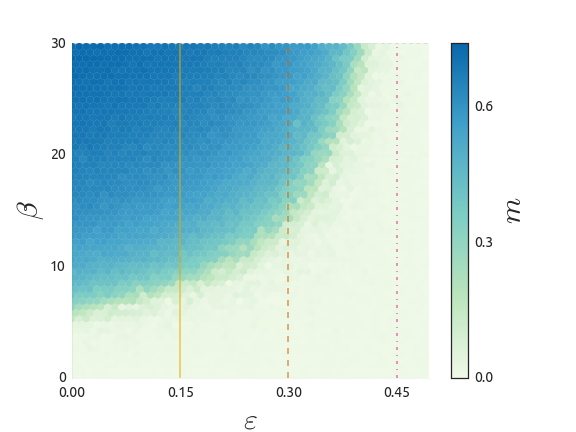
\includegraphics[scale=1.0]{mc-phase-diagram-eps.png}
    \caption{Diagrama de fases do consenso $m$ no plano $\beta \times   \varepsilon$, para desconfiança $\rho = 0.5$.}
\end{figure}
\begin{marginfigure}[-8cm]
    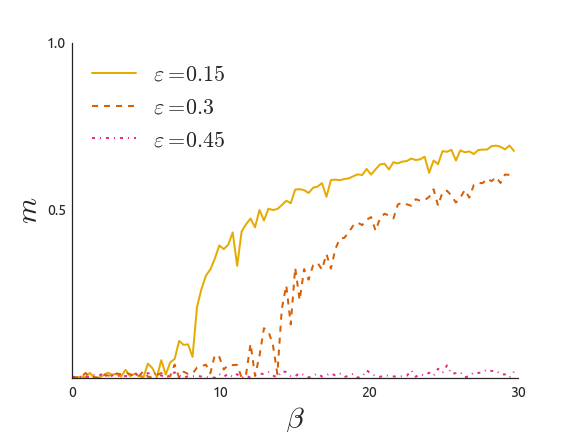
\includegraphics[scale=1.5]{mc-m-curves-eps.png}
    \caption{Curvas de consenso correspondentes às retas verticais na figura \ref{fig:mc-pd-eps}.}
\end{marginfigure}
Essa característica não foi capturada pela aproximação de campo médio, o que explica as diferenças entre as figuras \ref{fig:pd-ferro-eps} e \ref{fig:mc-pd-eps}.
Entretanto, a previsão de que apenas a desconfiança não é capaz de produzir grupos de opiniões distintas é corroborada, devido tamanha similaridade entre $\rho$ e $\ns$ no aparecimento de consenso, o que justifica nossa investida em mecanismos alternativos para tentar entender esse fenômeno.

\subsection{Um Retrato (Estatístico) da Semelhança Entre Agentes}

Outra forma interessante de ver o fenômeno de consenso é através dos histogramas de similaridade $\psi_{ij}$ definida por
\begin{align}
    \psi_{ij} & = \frac{1}{K} \agt{i}\cdot \agt{j} \label{eq:psi-ij}
\end{align}
que nada mais é do que o cosseno do ângulo formado pelos vetores cognitivos dos agentes $i$ e $j$.
De acordo com os diagrama nas figuras \ref{fig:mc-pd-rho} e \ref{fig:mc-pd-eps}, a sociedade tem duas fases, uma desordenada e uma de consenso.
Essas fases são reflexo da distribuição das opiniões a respeito de $\qst$, que estão diretamente relacionadas com $\psi_{ij}$, e portanto devem ser visíveis nos histogramas de similaridade.

\begin{figure}[h!]\label{fig:mc-cons-hist-br}
    \centering
    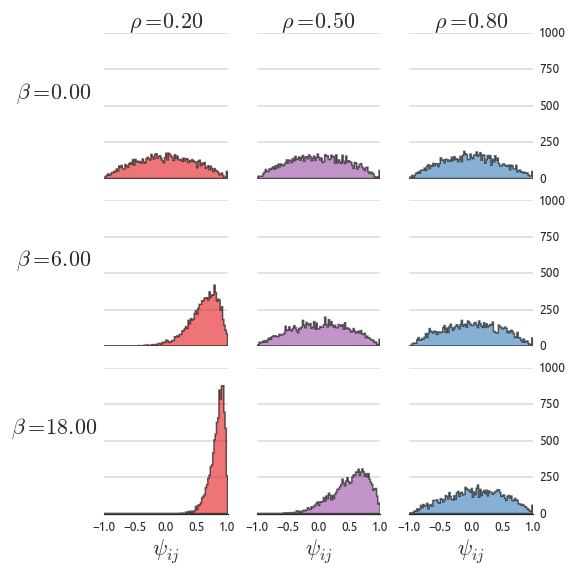
\includegraphics[scale=1.0]{mc-cons-hist-rb.png}
    \caption{Histogramas da similaridade $\psi_{ij}$ para alguns valores do estilo cognitivo $\rho$ e da pressão social $\beta$ com desconfiança $\ns=0$ fixa no modelo para o surgimento de consenso.}
\end{figure}

As figuras \ref{fig:mc-cons-hist-br} e \ref{fig:mc-cons-hist-be} mostram que conforme a pressão social aumenta, e a sociedade caminha para um consenso, a média dos histogramas de semelhança caminha em direção ao valor $1$, e a variância em torno da média vai diminuindo.
A intensidade desse fenômeno está relacionada com os valores do estilo cognitivo $\rho$ e da desconfiança $\ns$, sendo mais perceptível conforme menores seus valores.
Essa característica de baixos valores de $\rho$ estarem associados com uma menor flutuação tolerada nas opiniões é associada com um comportamento conservador, como mostrado em \parencite{Cesar2014,Vicente2014,Caticha2011}.
\begin{figure}[h!]\label{fig:mc-cons-hist-be}
    \centering
    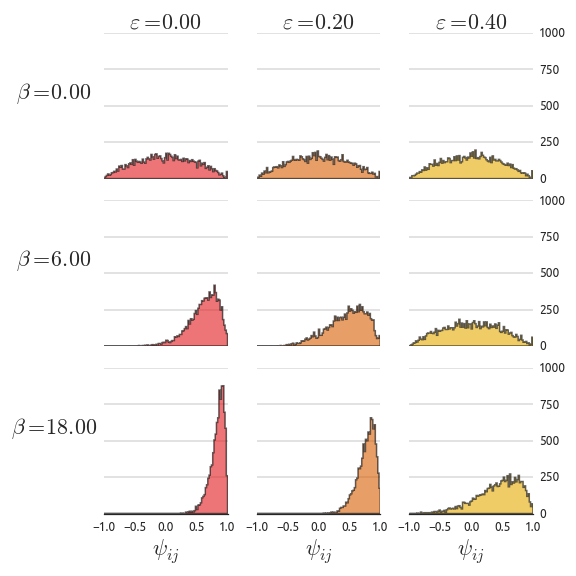
\includegraphics[scale=1.0]{mc-cons-hist-eb.png}
    \caption{Histogramas da similaridade $\psi_{ij}$ para alguns valores da desconfiança $\ns$ e da pressão social $\beta$ com estilo cognitivo $\rho=0.2$ fixo no modelo para o surgimento de consenso.}
\end{figure}

\section{Uma Dinâmica para as Relações Sociais}
\label{sec:DRS}

Um efeito colateral da interação dos agentes, não contemplado pelo modelo acima, é a evolução das relações sociais.
As próximas perguntas que nos fazemos são \emph{``como a escolha de parceiros sociais pode ser feita pelos agentes?''} e \emph{``como essa escolha afeta as fases de desordem e consenso na sociedade?''}.
Para respondê-las, implementaremos um mecanismo de controle das relações baseados nos choques de opinião.
Isso é feito definindo equações para $R_{ij}$ em função das opiniões dos agentes $i$ e $j$.

Restringindo entre $0$ e $1$ os valores de $R_{ij}$, e interpretando o valor nulo como indicativo do agente $i$ não considerar o agente $j$ como parceiro.\footnote{Estamos lidando com um grafo direcionado, representando possíveis não reciprocidades em relações entre agentes.}
A evolução de $R_{ij}$ é dada pela equação \eqref{eq:Rt},
\begin{align}
  R_{ij}(t+1) & = R_{ij} + \lambda\,R_{ij}(1-R_{ij})\sgn\inpr{h_i\,h_j}, \label{eq:Rijt}
\end{align}
fazendo nulo o termo de esquecimento, ou seja $\varphi = 0$.

As relações sociais $R_{ij}$ determinam a probabilidade $p(j|i)$ de cada parceiro $j$ ser escolhido pelo parceiro $i$ nessa rodada.
A escolha mais simples que podemos fazer para relacionar $R_{ij}$ e $p(j|i)$ é a seguinte
\begin{align}
  p(j|i) & = \frac{R_{ij}}{\sum_{k}R_{ik}}, \label{eq:pij-linear}
\end{align}
que pode ser interpretada diretamente como uma medida de distância \footnotemark entre os agentes $i$ e $j$. \footnotetext{na verdade seria o inverso da distância, dado que agentes interagem tem probabilidade nula de interação quando sua relação é também nula.}
A simulação de Monte Carlo é feita de modo análogo ao caso anterior, no qual as relações sociais estavam fixas, com a exceção da escolha do par $(ij)$ ser feita usando a probabilidade $p(j|i)$.

Apenas ajustar a probabilidade de interação entre os agentes não é capaz de produzir polarização de forma consistente.
Com a finalidade de produzir esse efeito, vamos definir a constante de $J_{ij}$, em analogia com o modelo \emph{'antiferromagnético'} usado para o campo médio no capítulo \ref{ch:C2}, mas desta vez como uma função explícita da relações sociais
\begin{align}
    J_{ij} & = \frac{1}{K}\,\sgn\inpr{R_{ij} - \half} \label{eq:Jij-Rij}
\end{align}

Definida dessa maneira, a grandeza $J_{ij}$ direciona o agente $i$ no sentido de aprender a opinião de $j$, caso sua relação esteja \emph{'acima da média'}, ou no sentido de se opor a $j$, caso esteja abaixo.
Por \emph{'acima da média'} entenda que o agente $i$ prefere interagir com $j$ mais do que com outros agentes.

\subsection{Complexidade no Nível das Opiniões}

O primeiro resultado dessa dinâmica pode ser observado através de histogramas da \emph{semelhança}, $\psi_{ij}$ \footnote{definida pela equação \eqref{eq:psi-ij}}.
Para interpretar os histogramas, consideraremos três possíveis situações de equilíbrio da sociedade.

Considere, primeiramente, a situação com baixa ou nula pressão social, $\beta$, indicando que o custo cognitivo da discordância é baixo.
Neste caso, não esperamos que os agentes aprendam as opiniões de seus parceiros e, portanto, nenhum consenso pode ser atingido.
Essa situação é a que ocorre na região clara dos diagramas de fases nas figuras \ref{fig:mc-pd-rho} e \ref{fig:mc-pd-eps}.
Neste caso, os vetores cognitivos dos agentes estarão distribuídos de maneira uniforme na $K$-esfera, e a semelhança entre eles terá média e moda nulas.

Na situação representada pela região escura dos diagramas de fases acima, representando as regiões de consenso, a situação é oposta.
O custo de discordar de um parceiro é elevado, dada a alta pressão social, de modo que os agentes são levados a aprender a opinião uns dos outros.
Isso conduz a uma distribuição de vetores bem mais localizada ao redor do questão $\qst$ ou sua oposta $-\qst$ .
A semelhança entre os agentes terá, portanto, média e moda próximos de $1$, de acordo com os valores do estilo cognitivo $\rho$ e da desconfiança $\ns$.
Esse é o caso em que representa os histogramas nas figuras \ref{fig:mc-cons-hist-br} e \ref{fig:mc-cons-hist-be} da seção anterior.

A terceira situação, que é a novidade desse modelo, é uma em que opiniões opostas em relação à $\qst$ podem coexistir.
É claro que para isso, é necessário uma pressão crítica grande o bastante para que o aprendizado seja necessário, como na situação de consenso.
Entretanto, dada a possibilidade de eliminar relações com agentes que discordam permite que opiniões opostas se mantenham, até que o consenso seja atingido em cada uma delas separadamente de modo que há uma rivalidade global.
Nesse caso, a semelhança entre os agentes também terá média nula, mas apresentará duas modas, cada uma tendendo a $\pm 1$, que indica que uma fração dos agentes compartilha opiniões semelhantes mas opostas a uma outra fração da sociedade.

%% \pagebreak
\begin{figure}[h!]\label{fig:mc-hist-br}
  \centering
  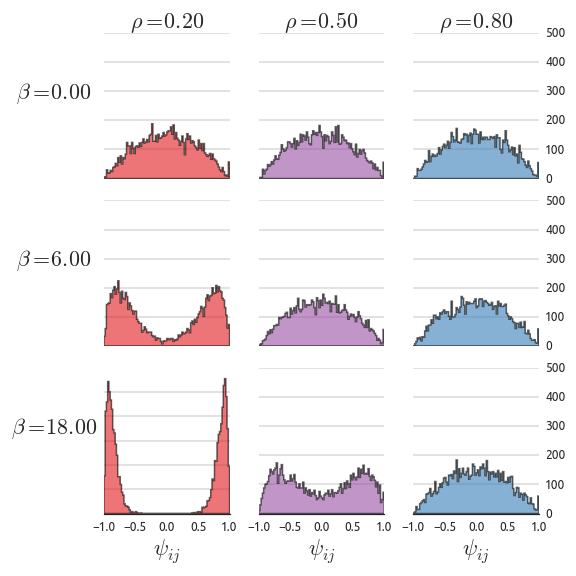
\includegraphics[scale=1.0]{mc-histograms-rhoxbeta.png}
  \caption{Histogramas da similaridade $\psi_{ij}$ para alguns valores do estilo cognitivo $\rho$ e da pressão social $\beta$ com desconfiança $\ns=0$ fixa no modelo com a dinâmica das relações sociais.}
\end{figure}
%% \pagebreak

As três situações acima são ilustrativas e diversos estados intermediários podem surgir, dependendo dos parâmetros que controlam o sistema.
As assinaturas estatísticas dessas situações ajudam, porém, a interpretar as fases da sociedade com relação à dinâmica das relações sociais.

A figura \ref{fig:mc-hist-br} mostra os histogramas de similaridade em diferente condições de estilo cognitivo $\rho$ e pressão social $\beta$, mantendo fixado o valor da desconfiança $\ns=0$.
Note que estilos cognitivos mais conservadores, dados por valores mais baixos de $\rho$, experimentam polarização em condições mais brandas de pressão social e desconfiança.

%% \pagebreak
\begin{figure}[h!]\label{fig:mc-hist-be}
    \centering
    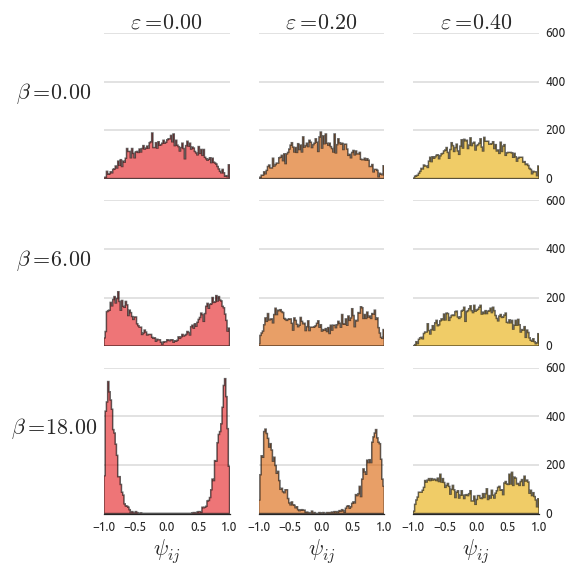
\includegraphics[scale=1.0]{mc-histograms-epsxbeta.png}
    \caption{Histogramas da similaridade $\psi_{ij}$ para alguns valores da desconfiança $\ns$ e da pressão social $\beta$ com estilo cognitivo $\rho=0.2$ fixo no modelo com a dinâmica das relações sociais.}
\end{figure}
%% \pagebreak

A figura \ref{fig:mc-hist-be} mostra histogramas análogos, desta vez em função da desconfiança $\ns$ e da pressão social $\beta$.
Note que a influência da desconfiança sobre o comportamento dos regimes de dissenso, polarização e consenso é similar à do estilo cognitivo, no sentido de dificultar o consenso conforme seu valor aumenta.

É evidente que a distribuição de opiniões com relação a $\qst$ está diretamente relacionada com os histogramas das figuras \ref{fig:mc-hist-br} e \ref{fig:mc-hist-be}.
Com isso podemos concluir que a sociedade tem duas \emph{'regiões de opinião'}, em contraposição à situação de consenso.
Do ponto de vista da teoria de aprendizado de máquina, podemos dizer que uma sociedade polarizada apresenta uma maior complexidade do que no estado de consenso.

\subsection{O Efeito da Dinâmica no Tecido Social}

Outro aspecto dessa complexidade pode ser observada nas matrizes das relações sociais.
Como apontado na seção anterior, as relações sociais formam, inicialmente, um grafo completo, ou seja todos os agentes são parceiros.
Conforme a sociedade evolui, relações podem ser fortalecidas ou destruídas de acordo com a concordância ou discordância dos agentes durante o encontro.

%% \pagebreak
\begin{figure}[h!]\label{fig:mat-br}
    \centering
    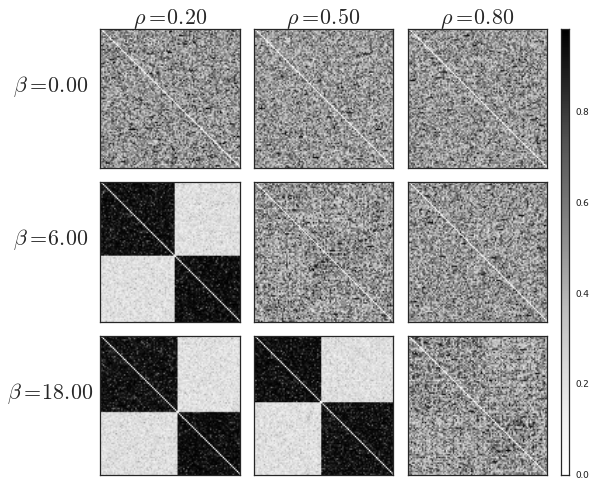
\includegraphics[scale=1.0]{mat-br.png}
    \caption{Matrizes das relações sociais $R_{ij}$ para alguns valores do estilo cognitivo $\rho$ e da pressão social $\beta$ com desconfiança $\ns=0.0$ fixo.}
\end{figure}
%% \pagebreak

Como é possível constatar olhando as figuras \ref{fig:mat-br} e \ref{fig:mc-hist-br}, conforme a distribuição de similaridade se torna mais estreita em relação às modas $\pm1$, estruturas mais evidentes são encontradas nas matrizes de relação social.
Isto é, na situação de polarização é possível observar dois blocos de relações sociais bem definidos, representando agente que interagem mais frequentemente com outros no mesmo bloco do que com agentes do outro bloco.
Essa é a noção de \emph{comunidade} no estudo de redes sociais \footcite{NewmanBook,Reichardt2008}. \footnote{As matrizes apresentadas nas figuras foram analisadas usando o algoritmo de \emph{SPIN} de \parencite{Tsafrir2005}, que reorganizas as linhas e colunas em uma matriz de distâncias de modo que linhas e colunas vizinhas representem menores distâncias.}

Em contraposição à estrutura de comunidade do estado polarizado, podemos observar um grafo completo, dado por uma matriz com um único bloco ou comunidade e relativo ao estado de consenso, ou um grafo aleatório, em que surge nenhuma comunidade e que representa a situação de dissenso nas figuras \ref{fig:mat-br} e \ref{fig:mat-be}.

%% \pagebreak
\begin{figure}[b!]\label{fig:mat-be}
  \centering
  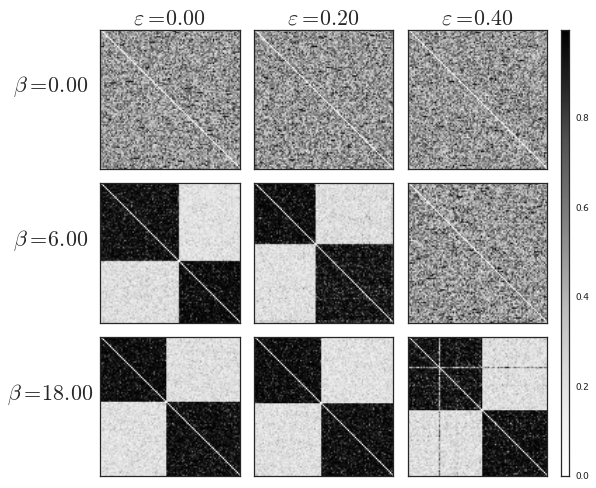
\includegraphics[scale=1.0]{mat-be.png}
  \caption{Matrizes das relações sociais $R_{ij}$ para alguns valores da desconfiança $\ns$ e da pressão social $\beta$ com estilo cognitivo $\rho=0.2$ fixo.}
\end{figure}
%% \pagebreak

Essa complexidade a nível de estrutura social é de uma natureza diferente da complexidade de opiniões.
Embora, por construção, as duas devam estar relacionadas, precisamos de uma forma de garantir que a influência do aprendizado social no estrutura das relações não é coincidência.

\subsection{Outra Forma de Ordem}

Para determinar a influência da opinião dos agentes na estrutura social, vamos introduzir um novo parâmetro de ordem
\begin{align}
    q & = \sum_{(ij)} \sgn\inbk{\inpr{R_{ij}-\half}h_ih_j} \label{eq:q-def}
\end{align}
Para entender como esse parâmetro nos permite associar o estado de polarização às estruturas de comunidade, considere apenas o termo da soma referente aos parceiros $i$ e $j$.

Se a relação $R_{ij}$ entre eles é boa, ou seja\footnote{que faz com que $J_{ij}=\frac{1}{K}$} $R_{ij} > \half$, então eles devem estar na mesma comunidade, e esperamos que a opinião deles tenha o mesmo sinal,  $h_ih_j>0$, no caso em que há polarização na sociedade.
Por outro lado, se eles não estão na mesma comunidade\footnote{fazendo com que $J_{ij}=-\frac{1}{K}$}, $R_{ij}<1/2$, quando há polarização esperamos que os agentes discordem, ou seja $h_ih_j < 0$.
Nesses dois casos, esse termo de $q$ será positivo, pois $\sgn \inbk{\inpr{R_{ij}-\half}h_ih_j}>0$.

Se, em oposição, os agente $i$ e $j$ estão na mesma comunidade mas discordam em opinião, ou concordam em opinião mas estão em comunidades distintas, esse termo será negativo.

O parâmetro $q$, que chamaremos de \emph{medida de estrutura}, é a média sobre todas a relações sociais dessa adequação entre opinião e comunidade, e pode ser vista justamente como um valor de quão bem definidas são as estruturas de comunidade.
Para chegar a essa conclusão basta perceber que o valor de $q$ será mais próximo de $1$ quão melhor for descrever os agentes com mesma opinião como uma comunidade e mais próximo de zero quando essa descrição não for boa.

\begin{figure}[h!]\label{fig:mc-q-curves-rb}
    \centering
    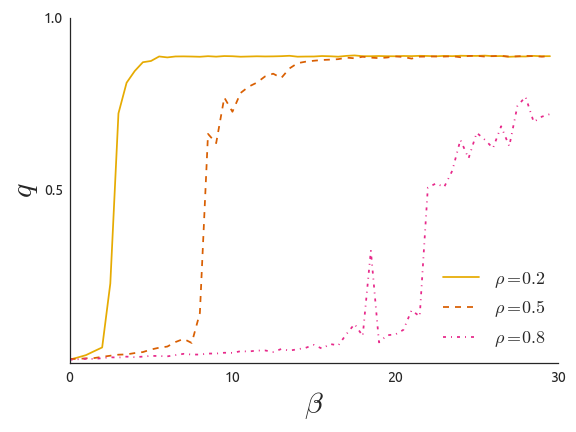
\includegraphics[scale=1.0]{mc-q-curves-rb.png}
    \caption{Curvas da medida de estrutura $q$ em função da pressão social $\beta$ para diferentes valores do estilo cognitivo $\rho$ e com desconfiança $\ns=0$ fixa.}
\end{figure}

As figuras \ref{fig:mc-q-curves-rb} e \ref{fig:mc-q-curves-eb} mostram uma transição entre as fases de desordem e polarização, semelhante à transição de fases na sociedade que atinge consenso.
De modo análogo aos resultados da seção \ref{sec:MCCT}, para valores de pressão social $\beta$ maiores que uma dada pressão crítica, que depende do estilo cognitivo $\rho$ e da desconfiança $\ns$, a sociedade experimenta uma fase em que comunidade de opinião bem formada coexistem.
Abaixo da pressão crítica, porém, não é possível atribuir a multitude de opiniões a comunidades bem estruturadas, e a sociedade vive uma fase de desordem.

\begin{figure}[h!]\label{fig:mc-q-curves-eb}
    \centering
    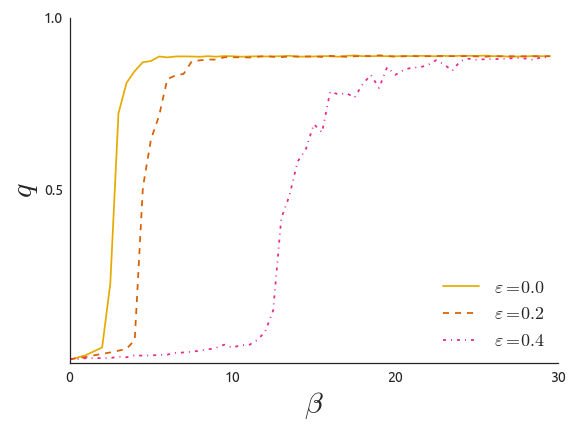
\includegraphics[scale=1.0]{mc-q-curves-eb.png}
    \caption{Curvas da medida de estrutura $q$ em função da pressão social $\beta$ para diferentes valores da desconfiança $\ns$ e com estilo cognitivo $\rho=0.2$ fixo.}
\end{figure}

O efeito do estilo cognitivo e da desconfiança na pressão crítica que possibilita a estruturação de comunidades é análogo ao caso de consenso.
Para valores de $\rho$ maiores, associados a agentes mais liberais, a formação de comunidades exige maior pressão social.
O mesmo pode ser dito sobre os valores de $\ns$.

Podemos ver como essa transição se dá ao longo da evolução da sociedade  tomando como exemplo a figura \ref{fig:mc-q-evol-r}, que mostra o valor de $q$ ao longo das interações entre agentes para alguns valores da pressão social $\beta$ e com $\rho$ e $\ns$ fixos.

\begin{figure}[b!]\label{fig:mc-q-evol-r}
    \centering
    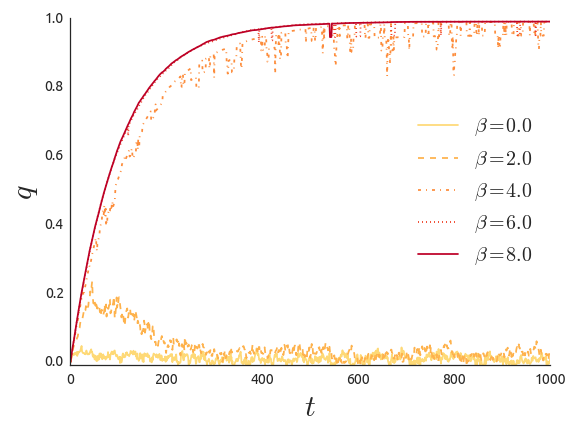
\includegraphics[scale=1.0]{mc-q-evol-r.png}
    \caption{Curvas da medida de estrutura $q$ em função do tempo $t$, em unidades de \emph{número médio de interações por agente}, para diferentes valores da pressão social $\beta$ e com desconfiança $\ns=0$ e com estilo cognitivo $\rho=0.2$ fixos.}
\end{figure}

É possível notar que, para baixos valores de pressão social, os valores de $q$ aumentam por um curto período de tempo, e convergem para zero em seguida.
Para valores mais altos de pressão, a medida de estrutura cresce até convergir para o valor $1$.
Com base na concepção de $q$ como uma medida da estruturação da sociedade, podemos interpretar esse resultado como uma espécie fenômeno que requer uma \emph{'massa crítica'}.
Isso é, as comunidades começam a se formar concomitantes com o aprendizado dos agentes, mas só se estruturam bem se uma porção suficiente de agentes compartilha opiniões mais concentradas.

Com a presente análise, concluímos que as habilidades de escolher o indivíduos com que um agente se relaciona e de escolher a natureza dessa relação são suficientes para criar complexidade social.
Essa complexidade diz respeito tanto à estrutura das relações sociais quanto à distribuição das opiniões e, de fato, é estabelecida como consequência do acoplamento entre as dinâmicas de aprendizado social e da relações entre agentes.
Os resultados apresentados nessa seção são novidade e proporcionam um modelo simples para a formação de estruturas sociais através de um vínculo direto entre a estrutura cognitiva dos agentes e sua interação social.

%% \newpage
\vfill
\pagebreak
\section{Jogos de Partidos}
\label{sec:DM}

Uma vez estabelecida uma dinâmica para as relações sociais que possibilitam o surgimento de grupos com opiniões distintas, podemos nos perguntar como a coexistência desses grupos é afetada por mudanças na pressão social e nas relações entre grupos.
Um  nicho social interessante para estudar a influencia da estrutura e das relações de poder é o das votações parlamentares de um governo democrático.

Com base numa análise, que embora lúdica é bastante interessante, apresentada no \emph{blog} \emph{Todas as Configurações Possíveis} \footcite{MarinoBlog1, MarinoBlog2}, podemos nos perguntar como a mudança de um presidente pode afetar as votações no plenário.
A análise lá apresentada consiste da projeção nas componentes principais da matriz de correlação entre os voto de parlamentares, em várias votações de projetos de lei, ao longo de vários mandatos presidenciais.
O resultado mostra a forte tendencia de partidos como o PMDB em manter seu apoio a projetos da posição, enquanto partidos rivais como PT e PSDB se opõem sistemática e independentemente de quem está no governo.

Nossa ideia é usar a plataforma de aprendizado social e estrutura de comunidade para tentar reproduzir esse comportamento.
Para isso, ao invés de considerar a multitude de partidos políticos no Brasil, lidaremos apenas com três partidos, que vivenciam uma troca de partido no poder ao longo de dois mandatos presidenciais.

\subsection{Um Modelo para a Influência Política}

O cenário é estabelecido com dois \emph{partidos ideológicos} formados por agentes concentrados ao redor de suas respectivas \emph{agendas}, representando os parlamentares de partidos rivais e os quais chamaremos  $A$ e $B$.
Um terceiro partido, ao qual damos o rótulo $C$, sem uma ideologia fixada integra o plenário e participa das votações.
As agendas políticas dos partidos serão denotadas por $\qst_A$ e $\qst_B$.

Sendo rivais, os integrantes dos partidos $A$ e $B$ não procuram uns aos outros para discutir projetos.
Essa situação é bem descrita pela fase de polarização com duas comunidades estudada na seção anterior.
Além disso, esses dois partidos têm ideologias fortes, de modo que eles não aceitam as opiniões dos integrantes do partido $C$ e com isso os integrantes dos partidos $A$ e $B$ discutem apenas entre si.
\begin{figure}[t!]\label{fig:parties-mat}
    \centering
    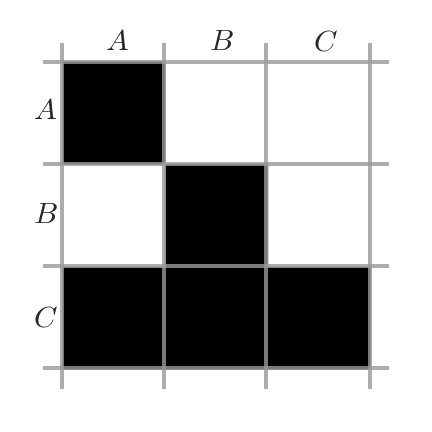
\includegraphics[scale=1.0]{parties-mat.png}
    \caption{Matriz das relações partidárias no modelo com três partidos.}
\end{figure}
O partido $C$, por outro lado, não tem ideologia e se permite interagir com qualquer parlamentar.
Para representar essa estrutura, criamos uma matriz de adjacência, a nível ultra métrico, que representa as possíveis interações entre parlamentares de acordo com seus partidos, ilustrada da figura \ref{fig:parties-mat}

Não estamos, neste momento, preocupados com a formação dos partidos e vamos supor que no período considerado nenhum parlamentar troca de partido, de modo que a estrutura da figura \ref{fig:parties-mat} é fixa.

A dinâmica de aprendizado é similar à usada nos cenários de sociedade com consenso ou polarização, com a exceção de não existir apenas uma questão.
De fato, as agendas política dos partidos $A$ e $B$ representam os projetos propostos por esses partidos e serão, portanto, as questões a serem discutidas pelos agentes.
Vamos convencionar que os parlamentares dos partidos $A$ e $B$ discutem apenas as agendas de seus partidos, enquanto os parlamentares de $C$ escolhem uniformemente entre as duas agendas quando procuram a opinião de outro agente, sendo que quem decide a agenda discutida é o agente que faz o papel de \emph{"professor"}.

Com relação ao estilo cognitivo dos parlamentares, temos que escolher considerar as possíveis diferenças com respeito a políticas liberais ou conservadoras ou considerar os parlamentares com uma mesma orientação nesse sentido.
Esse ponto é delicado e difícil de justificar sem um estudo mais profundo sobre esse aspecto da política brasileira, sendo nenhum de conhecimento do autor.
Por esse motivo, vamos escolher o mais simples, todos os parlamentares são semelhantes em estilo cognitivo.

Em se tratando de política, é certamente um disparate afirmar que não há desconfiança com relação às posições dos parlamentares com relação aos projetos em tramitação.
Entretanto, os resultados que apresentamos até então mostram que o efeito da desconfiança nos regimes da sociedade é similar ao do estilo cognitivo, a saber dificultar o aparecimento de estruturas de ordem.
É com isso em mente que vamos fixar $\ns=0$ nesse modelo, numa forma talvez inadequada de incluir os efeitos da desconfiança no estilo cognitivo\footnote{Outro ponto delicado, mas não completamente sem fundamento.
Para compreender melhor a motivação para isso, basta comparar os gráficos da função de modulação \eqref{eq:f-bayes} para diferentes valores de $\rho$ e $\ns$ e constatar que, com algumas restrições, aumentar $\rho$ é qualitativamente equivalente a reduzir $\ns$ e vice versa, de modo que determinar cada um independentemente não é trivial}.

O papel da pressão social nesse contexto precisa ser revisto.
Lembrando das fases de uma sociedade onde consenso pode surgir, parece natural que dentro de cada partido o valor de $\beta$ deva estar acima da pressão crítica necessária para atingir o consenso.
Porém, não é possível definir de forma heurística o regime no plenário como um todo porque, embora os partidos $A$ e $B$ estejam \emph{'isolados'} e em consenso, o partido $C$ pode mudar de opinião ou, melhor dizendo, posicionamento.
A capacidade de um partido influenciar o outro deve estar relacionada com seu  \emph{'poder político'}.
Vamos então associar o poder político do partido com relação à presidência, ou seja, o partido que estiver no governo deve ter mais poder para pressionar os parlamentares do que aquele que os demais.
Digamos que os poderes políticos do \emph{governo} e da \emph{oposição} são dados por $J_G$ e $J_O$ com $J_G > J_O$.
A \emph{pressão política} será a pressão social efetiva $\beta J_{ij}$, onde
\begin{align}
    J_{ij} & = \begin{cases}
        J_O & \text{se $j$ não faz parte do partido do governo}\\
        J_G & \text{se $j$ faz parte do partido do governo}
\end{cases}
\end{align}

Os partidos  viverão dois mandatos de mesma duração, sendo o primeiro sob o governo do partido $A$ e o segundo sob o governo do partido $B$.
A transição de governo é representada pela troca dos valores de $J_{ij}$.
Para tornar as coisas interessantes, e de certa forma próximas da situação real, vamos assumir que o número de parlamentares do partido $C$ é maior que os dos partidos $A$ e $B$.
A pergunta que queremos responder é: como o partido $C$ se comporta com relação às agendas de $A$ e $B$? Ou, em outras palavras, qual dos partidos rivais recebe o apoio do partido $C$?

Para respondê-la, consideramos duas situações distintas com relação à pressão social $\beta$ no plenário.
Numa delas, a oposição não tem coesão mas o governo tem, ou seja o valor de $\beta$ está abaixo da pressão crítica de modo que a pressão política da oposição não esteja acima da crítica, mas a do governo sim.
Na outra, $\beta$ está acima da pressão crítica, e tanto governo quanto oposição são coerentes, embora o governo exerça uma pressão política muito maior.

\begin{figure}[t!]\label{fig:mc-election-low-b}
    \centering
    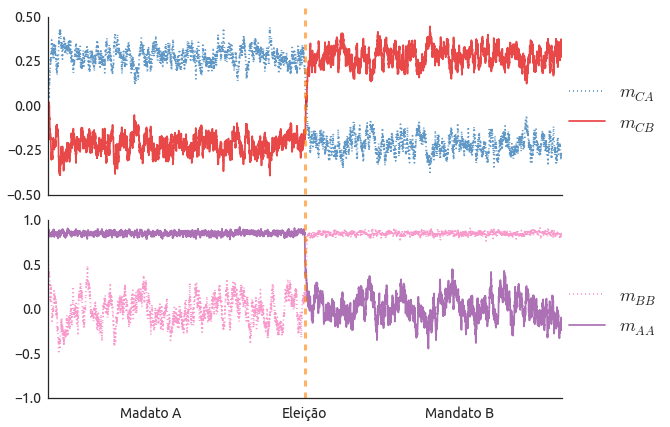
\includegraphics[scale=1.0]{mc-election-low-b.png}
    \caption{Evolução da adesão $m_{rs}$ às agendas $s$ pelo partido $r$ ao longo de dois mandatos com pressão social $\beta=1$ fixo.
    Os parâmetros $J_G=10$ e $J_O=1$ são atribuídos de acordo com o mandato. Os partidos tem tamanho $n_A=n_B=25$ e $n_C=100$ e a eleição ocorre em $t=5000$.}
\end{figure}

A resposta para essa pergunta pode ser obtida olhando para a evolução da \emph{adesão} $m_{rs}$, com $r,s \in \{A,B,C\}$, definida como a média das opiniões dos agentes do partido $r$ sobre a agenda do partido $s$.
Pela construção do modelo, as adesões interessantes serão $m_{CA}$, $m_{CB}$, $m_{AA}$ e $m_{BB}$, pois queremos saber o posicionamento do partido $C$ e devemos monitorar os outros partidos para saber como se comportam com relação às próprias agendas.

\begin{figure}[t!]\label{fig:mc-election-high-b}
    \centering
    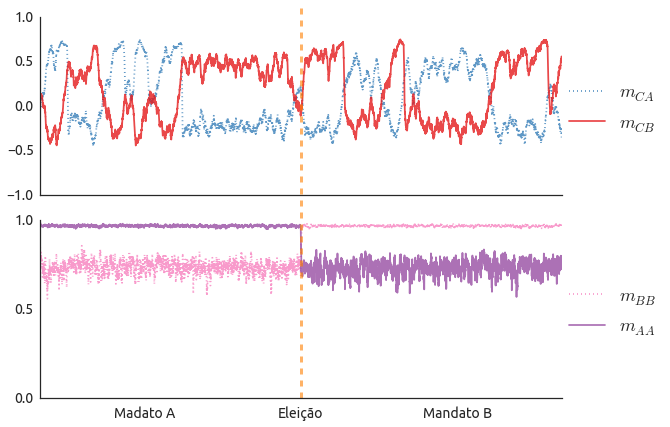
\includegraphics[scale=1.0]{mc-election-high-b.png}
    \caption{Evolução da adesão $m_{rs}$ às agendas $s$ pelo partido $r$ ao longo de dois mandatos com pressão social $\beta=5$ fixo.
Os parâmetros $J_G=50$ e $J_O=1$ são atribuídos de acordo com o mandato. Os partidos tem tamanho $n_A=n_B=25$ e $n_C=100$ e a eleição ocorre em $t=5000$.}
\end{figure}

A figura \ref{fig:mc-election-low-b}, quando a pressão social está abaixo da pressão crítica, mostra que, embora o partido $B$ comece concentrado, a falta de coesão faz com que se desprenda da sua agenda e o mesmo ocorre quando $A$ deixa de ser governo e passa a ser oposição.
Nesse caso, não temos partidos ideológico ao longo dos dois mandatos.
Por conta disso, o partido $C$ acaba apoiando o governo, seja do partido $A$ ou do partido $B$.

No caso de pressão acima da pressão crítica, ilustrada na figura \ref{fig:mc-election-high-b}, é possível perceber que os partidos rivais $A$ e $B$ continuam focados em suas agendas, embora sofram um pequeno abalo no valor absoluto do consenso quando não estão no governo.
Por outro lado, a adesão do partido $C$ oscila entre governo e oposição, de modo que seu apoio não é tão óbvio quanto no caso da pressão abaixo da crítica.
Esse resultado é sensível ao tamanho relativo dos partidos e da relação de poder entre governo e oposição, podendo não ser observado caso a diferença de poder não seja muito grande ou caso os partidos sejam distribuídos de forma mais justa ou com a maioria em um dos partidos ideológicos.
Todavia, esse resultado reproduz parte do comportamento observado nos deputados em votações ao longo dos mandatos dos ex-presidentes \emph{Fernando Henrique Cardoso} e \emph{Luiz Inácio Lula da Silva}, como veremos a seguir.
Embora a confirmação experimental ainda não seja possível, podemos ter uma ideia de quais elementos do modelo providenciam uma explicação qualitativa do comportamento político no congresso nacional.

\subsection{Uma Análise das Votações em Plenário ou\\
            `A Valsa dos Partidos` no Brasil}

%% inserir análise experimental

Como mencionado na seção anterior, a análise dos resultados de votações em plenário ao longo dos mandatos presidenciais realizada por \emph{R. Marino} em seu \emph{`blog`} inspirou a elaboração do modelo de agentes apresentado acima.
A aquisição dos dados foi feita através das páginas mantidas pelos parlamentares ou através de requerimento direto à assessoria da câmara.

Esses dados consistem das informações sobre o projeto de lei sendo votado, o dia da votação, além do nome, do voto, do partido de filiação e do estado de cada parlamentar votante.
A análise presente em \parencite{MarinoBlog1, MarinoBlog2} consiste na visualização da evolução na projeção de duas componentes principais da matriz de correlação desses votos, identificados pelos partidos.
Felizmente, os dados estão acessíveis nestes sítios.

O que fizemos foi pegar os dados disponíveis e identificar a concordância média entre os votos do \emph{PMDB} e do \emph{PSDB} e entre os votos do \emph{PMDB} e do \emph{PT}, bem como a coesão entre os votos do \emph{PT} e \emph{PSDB}, ao longo dos dois mandatos do \emph{FHC} e dos dois mandatos do \emph{Lula}.
Embora a concordância entre dois deputados em relação à um dado projeto de lei não seja idêntico ao que foi chamado de adesão, $m_{rs}$, na elaboração do modelo, é evidente que estão diretamente relacionadas, de modo que trataremos a concordância como se fosse a adesão.

Note, porém, que não temos como determinar a pressão social à qual a câmara estaria submetida ou a influência política do partido no governo.
Podemos, no máximo, comparar os dados com os cenários ilustrados pelo modelo e ver quais características do modelo podem fazer algum sentido.
\begin{figure}[t!]\label{fig:dados-marino}
    \centering
    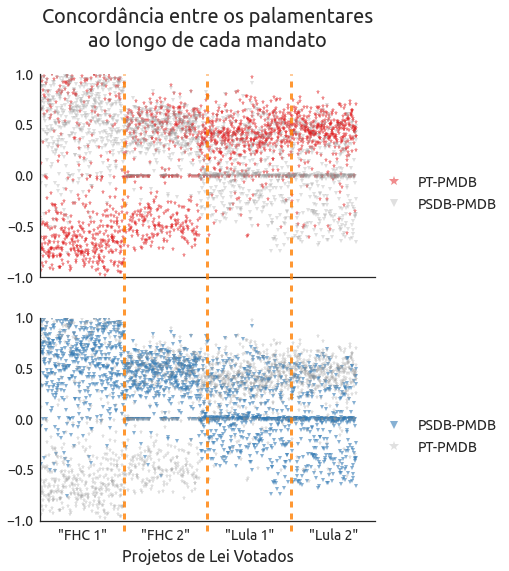
\includegraphics[scale=1.0]{dados-marino.png}
    \caption{Evolução da concordância nos votos em câmara dos deputados do \emph{PMDB} com os deputados do \emph{PSDB} ou \emph{PT} ao longo dos mandatos de \emph{FHC} e \emph{Lula}.}
\end{figure}

A figura \ref{fig:dados-marino} mostra a mudança no comportamento da concordância entre os deputados do \emph{PMDB} com os partidos no poder ou na oposição. \footnote{Os resultados apresentados nessa seção, diferente da análise feita em \parencite{MarinoBlog1}, não fez uso de nenhum pré-processamento dos dados.}
É possível notar que o apoio do \emph{PMDB} está sempre mais concentrado no partido que está na presidência, mudando de forma quase abrupta na transição de governo que se deu entre \emph{FHC} e \emph{Lula}.
Nesse gráfico, cada ponto é a média da concordância entre todos os deputados do \emph{PMDB} com todos aqueles do \emph{PSDB} (em azul) ou do \emph{PT} (em vermelho) para um dado projeto de lei em votação, ordenados pela data.
\begin{figure}[t!]\label{fig:dados-marino-medias}
    \centering
    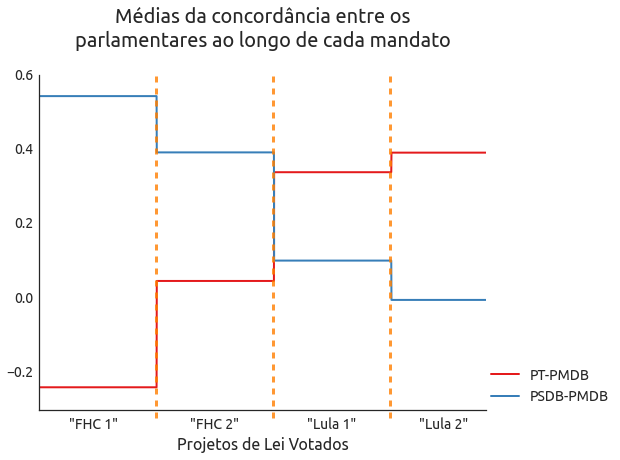
\includegraphics[scale=1.0]{dados-marino-medias.png}
    \caption{Evolução da média das concordância nos votos em câmara dos deputados do \emph{PMDB} com os deputados do \emph{PSDB} ou \emph{PT} ao longo dos mandatos de \emph{FHC} e \emph{Lula}.
Essa figura ilustra o apoio médio do \emph{PMDB} em cada mandato considerado.}
\end{figure}

A figura \ref{fig:dados-marino-medias} facilita a visualização substituindo cada ponto pela média sobre o mandato.
Embora a média não seja um bom representativo, dado que somente o número de projetos de lei apoiados não representa completamente as conquistas políticas \footnote{Alguns projetos podem ser mais importantes que outros na realização da agenda política de cada partido, então se um partido consegue o apoio necessário em projetos importantes, mesmo que em menor número, pode não estar de fato sofrendo uma oposição.}, o comportamento da média no segundo mandato do \emph{FHC} e no primeiro do \emph{Lula} exibem o mesmo comportamento do modelo no cenário de pressão abaixo da crítica.
Isso pode indicar qual a influência política do partido no governo é mais relevante do que a pressão política na câmara em si.

Entretanto, ao verificarmos a evolução da coesão interna do partidos \emph{`rivais`}, \emph{PSDB} e \emph{PT}, percebemos que nenhum dos cenários estabelecidos pelo modelo explica bem o comportamento observado nos dados.
Como visto na figura \ref{fig:dados-marino-coesao}, tanto \emph{PT} quanto \emph{PSDB} passam por um enfraquecimento na coesão ao longo dos quatro mandatos considerados.
\begin{figure}[t!]\label{fig:dados-marino-coesao}
    \centering
    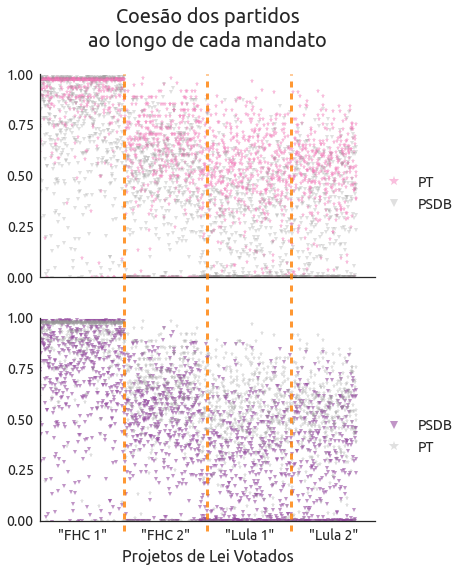
\includegraphics[scale=1.0]{dados-marino-coesao.png}
    \caption{Evolução da coesão interna do \emph{PSDB} ou \emph{PT}, observada através dos votos dos deputados em câmara, ao longo dos mandatos de \emph{FHC} e \emph{Lula}.}
\end{figure}

Novamente, é mais fácil olhar apenas para a média sobre cada mandato para visualizar mais facilmente esse comportamento, que é completamente distinto do produzido pelo modelo.
Isso nos diz que o modelo faz hipóteses inadequadas sobre algum aspecto do comportamento político, e precisa ser refinado de alguma forma.
Embora mais estudo nessa direção seja necessário, o autor acredita que as hipóteses que devam ser atacadas sejam a de isolamento do partidos rivais e a natureza estática da agenda de cada partido, embora a imposição de um único estilo cognitivo a todos os agentes, independente do partido, possivelmente tenha uma influência notável.
\begin{figure}[t!]\label{fig:dados-marino-coesao-medias}
    \centering
    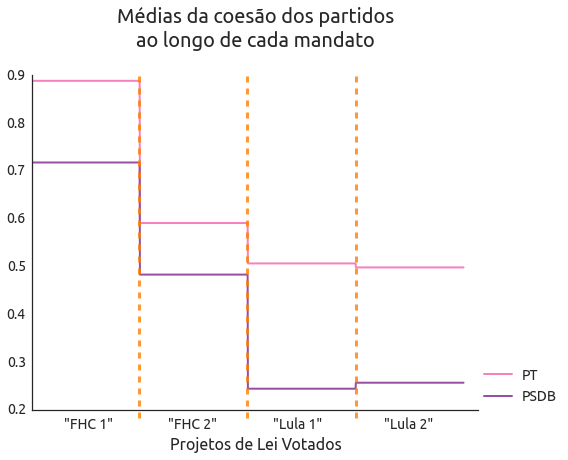
\includegraphics[scale=1.0]{dados-marino-coesao-medias.png}
    \caption{Evolução da média da coesão interna do \emph{PSDB} ou \emph{PT}, observada através dos votos dos deputados em câmara, ao longo dos mandatos de \emph{FHC} e \emph{Lula}.}
\end{figure}

Com base nos dados apresentados, podemos concluir que o modelo de formação de opinião através da interação de agentes reproduz parte do comportamento político observado no plenário brasileiro.
Entretanto, a formação de coalizões, não tendo sido extensivamente estudada, talvez possa explicar as disparidade entre o modelo e a realidade.
Dito isso, o fato do modelo reproduzir algum comportamento observado é em si impressionante e nos proporciona uma base qualitativa de interpretação dos processos políticos, e talvez estejamos um passo mais perto da capacidade de compreendê-los o suficiente para fazer previsões.

Para finalizar, um comentário especulativo sobre os dados sobre o apoio do \emph{PMDB} e as eleições presidenciais.
Notem que do primeiro para o segundo governo \emph{FHC}, o \emph{PSDB} experimentou uma redução no apoio recebido pelo \emph{PMDB}.
Situação oposta à do \emph{PT} entre o primeiro e segundo mandatos do \emph{Lula}.
Dado que o \emph{PSDB} perdeu a eleição presidencial após o segundo governo \emph{FHC} e que o \emph{PT} ganhou a eleição presidencial após o segundo governo \emph{Lula}, será que é sensato questionar se há uma relação entre a capacidade de manter o poder e o apoio de partidos \emph{`maleáveis`}?
A capacidade de responder essa pergunta está além do que podemos fazer por enquanto, dada a juventude da democracia brasileira pós ditadura militar, mas fazer perguntas tolas são sempre uma boa maneira de incentivar uma investigação mais profunda.

% Neste capítulo concluímos que o mecanismo de formação de estrutura social proposto é capaz de introduzir complexidade nas relações sociais e na distribuição de opiniões.
% Vimos um exemplo de como fenômenos sociais, no caso as disputas políticas na câmara, podem ser possivelmente descritos através de um modelo preocupado em relacionar as características cognitivas aos fenômenos sociais\footnote{note que embora tenha sido apresentado de forma um tanto lúdica, o modelo para as votações em plenário acabou se mostrando impressionante em vários aspectos.}.


%% Capítulo 4
%%% Capítulo 4 - Conclusão e Discussão

\chapter{Conclusões e Futuros Estudos}
\label{ch:C4}

\section{Uma Breve Revisão dos Resultados}

Neste trabalho desenvolvemos modelos para o estudo de fenômenos sociais com base em características cognitivas dos humanos.
Como foi visto no capítulo \ref{ch:C1}, o crescente corpo de resultados a respeito do comportamento humano, tanto a nível neural quanto psicossocial nos guiam na captura dos elementos básico do comportamento social.
Estabelecida a base empírica e fazendo uso das técnicas da mecânica estatística e da teoria de aprendizado de máquina, fomos capazes de estabelecer uma dinâmica para o aprendizado social, que exerce papel fundamental na interpretação dos fenômenos exibidos pelos modelos.

No capítulo \ref{ch:C2} desenvolvemos a teoria elementar para a abordagem estatística de fenômenos de interação social através da troca de opiniões.
O uso de ferramentas, como o método de máxima entropia, nos permitiu compreender através da análise de campo médio qual seria o comportamento de agentes que aprendem em conjunto, bem como o de agentes que se antagonizam, em analogia com sistemas ferromagnéticos e antiferromagnéticos.
Note que, embora este trabalho tenha tomado como modelo base outros trabalhos recentes na mesma área \footcite{Cesar2014,Vicente2014,Caticha2011}, esta é a primeira vez que uma análise um pouco mais profunda é feita em relação à desconfiança $\ns$ ao desenvolver a sociedade baseada no custo cognitivo \eqref{eq:Vij}.

No capítulo \ref{ch:C3} conseguimos comparar os resultados de campo médio com simulações usando o custo cognitivo associado à função de modulação Bayesiana, reproduzindo os resultados encontrado nas referências.
Com base nesses resultados, elaboramos um modelo de construção (ou aniquilação) das relações sociais com base na troca de opiniões.
Esse modelo se mostrou capaz de produzir a estrutura de comunidade com distintas opiniões, proporcionando inclusive uma medida do grau de organização dessa estrutura.

Por fim, um pequeno modelo de comportamento do plenário brasileiro foi elaborado para ilustrar algumas das possibilidades ao utilizar a nossa abordagem no estudo de fenômenos reais.
Embora as bases sob as quais esse modelo foi construído demandem mais estudo, seus resultados são interessantes pela capacidade de reproduzir o comportamento observado nas votação em plenário.
Entretanto, esses resultados são tratados como um guia qualitativo e qualquer esperança de usar esse modelo para explicar quantitativamente fenômenos reais necessita de base experimental.

Além dos resultados apresentados, diversos pontos podem ser destacados com relação ao modelo utilizado.
A escolha de usar apenas uma questão é uma limitação que pode ser facilmente removida, embora o custo computacional envolvido é um preço alto a pagar.
A escolha da topologia da rede social como um grafo completo é irreal na maior parte das redes sociais.
Porém, como um dos focos do trabalho era a construção das estruturas sociais, a escolha de alguma topologia mais realista não é facilmente justificável.
Por fim, os resultados apresentados no capítulo \ref{ch:C3} dependem de parâmetros usado nas simulações de Monte Carlo para os quais há pouca margem para interpretação dentro do modelo.

Por exemplo, o raio do cone dentro do qual o vetor cognitivo de um agente pode ser proposto está associado com a velocidade de convergência do algoritmo e pode também ser associado a uma velocidade de aprendizado.
Porém, essa taxa não surge na dedução apresentada no capítulo \ref{ch:C2} e precisaria ser introduzida artificialmente tendo como justificativa seu uso no algoritmo.
Os resultados apresentados neste trabalho são aqueles mais robustos com relação a esses parâmetros, e diversas variações dos modelos que poderiam gerar outras interpretações para os fenômenos não foram apresentados por não estarem sob controle dos parâmetros fornecidos pela teoria.

\section{O que há pela frente?}

Embora o fenômeno de estruturação social possa ser um pouco melhor compreendido através dos resultados deste trabalho, diversas críticas podem ser feitas com relação à elaboração do modelo.
Esforço deve ser desempenhado no sentido de justificar a forma da dinâmica das relações sociais que, diferente da dinâmica de aprendizado, foi estabelecida de forma heurística.
Tal justificativa demanda não apenas uma análise matemática mais delicada das interações sociais como também de resultados experimentais diretamente relacionado a escolha de amigos ou de colegas de trabalho e outros comportamentos relacionados.

A falta do respaldo experimental é outra crítica que pode ser feita a este trabalho.
A busca de resultados em áreas bem estudadas do comportamento social é prioridade para a sequência do trabalho apresentado aqui.


%%%

%%% back matter
\backmatter
%% \selectlanguage{brazilian}
\printbibliography
% \printindex
%%%

\end{document}
